\documentclass[journal]{IEEEtran}
% Midsem B.Tech Project report. Build: tectonic main.tex  (or upload report/ to Overleaf, pdfLaTeX/XeLaTeX)
\usepackage{amsmath,amssymb}
\usepackage{graphicx}
\usepackage{booktabs}
\usepackage{multirow}
\usepackage{xcolor}
\usepackage{url}
\usepackage[hidelinks]{hyperref}
\usepackage{cite}
\usepackage{dblfloatfix}
\usepackage{placeins}      % \FloatBarrier: all figures before the references   % keep wide tables/figures in order
\graphicspath{{figures/}}
\newcommand{\missing}[1]{\textcolor{red}{[MISSING: #1]}}

\begin{document}

\title{Noise-Aware Transformer-Based Low-Light Image Enhancement with Downstream Object Detection Evaluation\\
\large Mid-Semester B.Tech Project Report}

\author{\missing{Student name}, \missing{Roll number}\\
Supervisor: \missing{Supervisor name and title}\\
Department of Electrical Engineering, Indian Institute of Technology Patna\\
\missing{Date}}

\maketitle

\begin{abstract}
Photographs taken in dim light are dark, noisy and colour-shifted, and simply brightening them amplifies the noise.
This report presents the first half of a project on transformer-based low-light image enhancement. We reproduce
Retinexformer, a one-stage Retinex-based transformer, together with classical, zero-shot, transformer and diffusion
baselines, and evaluate all of them under a single protocol: fidelity (PSNR, SSIM), perceptual distance (LPIPS),
no-reference quality (NIQE), quality in the darkest image regions, efficiency on one GPU, and usefulness for a
COCO-pretrained YOLOv8 detector on the ExDark dataset. The released Retinexformer weights reproduce the published
LOL-v1 result (25.15 vs.\ 25.16~dB), whereas re-training from scratch with the official configuration reaches
23.10~dB. We show that the published numbers of a diffusion baseline rely on a ground-truth brightness correction
worth 4--8.5~dB, that 91 of the 100 LOL-v2-real test images also appear in the LOL-v1 training set, and that no
enhancer improves zero-shot detection on ExDark (mAP50 0.662 on raw images vs.\ at most 0.603 after enhancement).
Finally, we test a noise-aware, SNR-weighted training loss in a controlled fine-tuning experiment. It yields a
consistent but very small gain in dark regions (13 of 15 test images, +0.02~dB on average) and no measurable gain
otherwise. We discuss why, and plan the second half of the project accordingly.
\end{abstract}

\begin{IEEEkeywords}
Low-light image enhancement, Retinex theory, vision transformer, signal-to-noise ratio, object detection, reproducibility.
\end{IEEEkeywords}

% =====================================================================================================
\section{Introduction}
\IEEEPARstart{C}{ameras} need light. When a scene is lit by a street lamp, a screen or a dim room, the sensor
collects few photons, so the recorded image is dark, has low contrast, and is dominated by sensor noise; artificial
light sources add colour casts and over-exposed spots. Such images are common in phone photography,
surveillance and driving, and they hurt not only human viewers but also computer-vision systems such as object
detectors~\cite{li2022survey,loh2019exdark}. Low-light image enhancement (LLIE) aims to turn such an input into an
image that looks as if it had been captured in good light.

Brightening alone is not enough. A gain applied to a dark pixel multiplies the noise in that pixel as much as the
signal, so the darkest regions---where the signal-to-noise ratio (SNR) is lowest---become the noisiest after
enhancement. Classical methods such as histogram equalization, CLAHE~\cite{zuiderveld1994clahe} and gamma
correction redistribute brightness without modelling noise, and Retinex-based optimization
methods~\cite{guo2017lime} rely on hand-crafted priors. Deep networks learn the mapping from data and now dominate
the field~\cite{li2022survey}; the most recent ones are transformers~\cite{xu2022snr,wang2023llformer,cai2023retinexformer}
and diffusion models~\cite{hou2023gsad,yi2023diffretinex}.

This project starts from Retinexformer~\cite{cai2023retinexformer}, a compact transformer that guides its attention
with an estimated illumination map. Retinexformer is aware of \emph{where the image is dark} but has no explicit
notion of \emph{how noisy} a region is, while the SNR-Aware method~\cite{xu2022snr} uses an SNR map but not the
Retinex framework. In addition, enhancement methods are usually ranked by PSNR and SSIM alone, although a growing use
of LLIE is as a pre-processing step for machines.

\subsection{Related Work}
\emph{Classical methods.} Histogram equalization spreads the intensity histogram over the full range; CLAHE does
so on small tiles with a clip limit to avoid over-enhancement~\cite{zuiderveld1994clahe}. Retinex theory models an
image as reflectance times illumination; LIME~\cite{guo2017lime} estimates and refines an illumination map. These
methods are training-free but ignore noise, which remains or is amplified.

\emph{Supervised CNNs and deep Retinex.} LLNet~\cite{lore2017llnet} used a stacked denoising autoencoder.
Retinex-Net~\cite{wei2018retinexnet} decomposes images into reflectance and illumination with sub-networks and
introduced the paired LOL dataset; KinD~\cite{zhang2019kind} adds a reflectance restoration stage; the
sparse-gradient network of Yang \emph{et al.} introduced LOL-v2~\cite{yang2021lolv2}; MIRNet~\cite{zamir2020mirnet}
is a general multi-scale restoration network. Chen \emph{et al.}~\cite{chen2018sid} learn directly from raw sensor
data. Supervised methods reach the highest scores but depend on paired data, which is hard to collect.

\emph{Unsupervised and zero-shot methods.} EnlightenGAN~\cite{jiang2021enlightengan} trains a GAN on unpaired
images. Zero-DCE~\cite{guo2020zerodce} predicts pixel-wise curves using only non-reference losses, RUAS~\cite{liu2021ruas}
unrolls a Retinex optimization with architecture search, and SCI~\cite{ma2022sci} learns a self-calibrated
illumination module that reduces to a few hundred parameters at test time. These methods generalize well and are
fast, but they do not denoise.

\emph{Transformers.} Self-attention~\cite{vaswani2017attention} relates every position to every other one, but its
cost grows quadratically with the number of tokens; restoration transformers therefore restrict attention to windows
(e.g. Swin~\cite{liu2021swin}) or compute it across channels (Restormer~\cite{zamir2022restormer}).
SNR-Aware~\cite{xu2022snr} combines a convolutional branch for high-SNR regions with a transformer branch for
low-SNR regions; LLFormer~\cite{wang2023llformer} targets ultra-high-definition images; Retinexformer~\cite{cai2023retinexformer}
places channel-wise attention guided by illumination features inside a one-stage Retinex framework.

\emph{Diffusion models.} GSAD~\cite{hou2023gsad} and Diff-Retinex~\cite{yi2023diffretinex} generate the enhanced
image by iterative denoising and produce realistic textures, at the price of many network evaluations per image.

\emph{Enhancement for detection.} Backlit and low-light enhancement has been used before recognition
tasks~\cite{bose2023luminet}, and Retinexformer reports detection on ExDark~\cite{loh2019exdark} with a YOLOv3 detector
trained from scratch on enhanced images. Whether enhancement helps an off-the-shelf detector trained on normal-light
images is less studied.

\emph{Research gap.} (i) Noise amplification in dark regions is still an open problem~\cite{li2022survey}.
(ii) Retinexformer is illumination-aware but not noise-aware. (iii) Methods are rarely compared under one evaluation
protocol that includes task-based and region-specific metrics. (iv) Diffusion models trade large speed costs for
quality, and their reported numbers are not always obtained under the same protocol as other methods.

\subsection{Contributions and Organization}
The work completed in the first half of the project is:
\begin{itemize}
\item A reproduction of Retinexformer and eight baselines---classical, zero-shot, transformer and diffusion---scored by
one script on three paired and three unpaired test sets, with every number matched against the original papers.
\item Two protocol findings: GSAD's test script rescales outputs to the ground-truth brightness (worth 4--8.5~dB), and
91 of the 100 LOL-v2-real test images are also LOL-v1 training images.
\item A detection study on ExDark showing that no enhancer improves a COCO-pretrained YOLOv8m.
\item A noise-aware, SNR-weighted loss and a controlled fine-tuning experiment (control vs.\ SNR loss vs.\ FFT loss vs.\
both), evaluated globally and in the darkest image regions.
\end{itemize}
Section~\ref{sec:background} gives background, Section~\ref{sec:method} the methods, Section~\ref{sec:setup} the
experimental setup and Section~\ref{sec:results} the results. Section~\ref{sec:discussion} discusses limitations,
Section~\ref{sec:plan} the plan for the second half, and Section~\ref{sec:conclusion} concludes.

% =====================================================================================================
\section{Background}\label{sec:background}
\subsection{Retinex Model}
Retinex theory describes an observed image $I\in\mathbb{R}^{H\times W\times 3}$ as the element-wise product of a
reflectance $R$, which holds the colours of the objects, and an illumination $L$, which holds the light falling on
them:
\begin{equation}
I = R \odot L. \label{eq:retinex}
\end{equation}
Enhancement can then be seen as estimating $L$ and replacing it by a brighter, more uniform illumination. In real
dark images, however, the sensor adds noise and compression adds artifacts, so neither $R$ nor $L$ is clean, and
dividing by a small $L$ amplifies the corruption.

\subsection{Self-Attention and Its Cost}
A transformer layer turns $N$ tokens $X\in\mathbb{R}^{N\times C}$ into queries $Q=XW_Q$, keys $K=XW_K$ and values
$V=XW_V$, and mixes the values with weights computed from query--key similarity:
\begin{equation}
\mathrm{Attn}(Q,K,V)=\mathrm{softmax}\!\left(QK^{\top}/\sqrt{d}\right)V, \label{eq:attn}
\end{equation}
where $d$ is the head dimension. The matrix $QK^{\top}$ is $N\times N$. If every pixel of a $600\times400$ LOL image
were a token, $N=240{,}000$ and the matrix would have $5.8\times10^{10}$ entries, which is infeasible. Computing the
attention across \emph{channels} instead, $\mathrm{softmax}(K^{\top}Q)\in\mathbb{R}^{C\times C}$, makes the cost grow
linearly with $N$; this is the choice made by Restormer~\cite{zamir2022restormer} and Retinexformer~\cite{cai2023retinexformer}.

% =====================================================================================================
\section{Methodology}\label{sec:method}
\subsection{Overview}
Fig.~\ref{fig:pipeline} summarizes the project: three groups of data, five families of enhancement methods, and six
evaluation axes. Every method is evaluated with the same scripts; the darkest-region metric and the detection metric
are added by this project.

\begin{figure}[t]
\centering
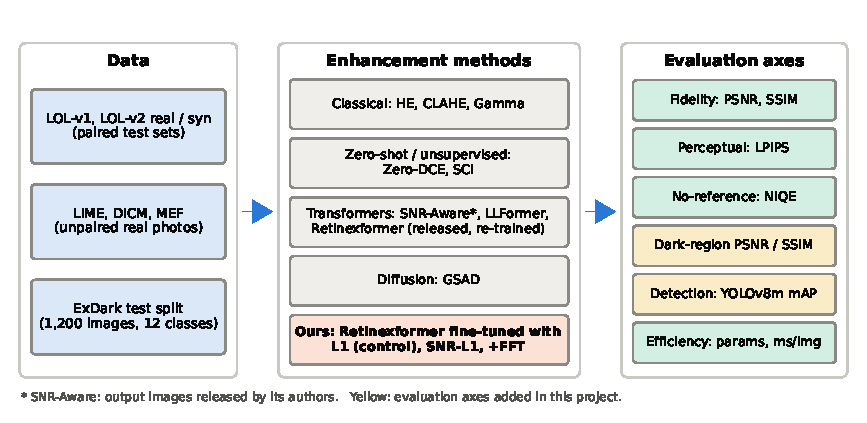
\includegraphics[width=\columnwidth]{pipeline.pdf}
\caption{Overview of the evaluation pipeline. Every enhancement method is scored on every evaluation axis that applies
to the data (paired metrics on LOL, NIQE on unpaired photos, detection on ExDark).}
\label{fig:pipeline}
\end{figure}

\subsection{Retinexformer}
Retinexformer~\cite{cai2023retinexformer} has two parts (Fig.~\ref{fig:arch}). We describe it as implemented in the
released code, with the configuration used for LOL (base width $C=40$, one stage, blocks $[1,2,2]$).

\emph{Illumination estimator.} The input $I$ and its channel mean are concatenated and passed through a $1\times1$
convolution and a $5\times5$ depth-wise convolution, giving light-up features $F_{lu}$; a final $1\times1$ convolution
gives a three-channel light-up map $\bar{L}$. The lit-up image is
\begin{equation}
I_{lu} = I \odot \bar{L} + I. \label{eq:lightup}
\end{equation}
$I_{lu}$ is brighter but still contains the noise and artifacts of $I$, now amplified.

\emph{Corruption restorer.} An Illumination-Guided Transformer (IGT) removes these corruptions. It is a two-level
U-shaped network: a $3\times3$ embedding, Illumination-Guided Attention Blocks (IGABs) at widths $C$, $2C$ and $4C$
with strided-convolution down-sampling and transposed-convolution up-sampling, skip connections, and a final $3\times3$
convolution whose output is added to $I_{lu}$. The light-up features $F_{lu}$ are down-sampled along with the image
features and fed to every block.

\emph{Illumination-guided attention.} Inside an IGAB, the features are projected to $Q$, $K$ and $V$; the values are
multiplied by the light-up features, $V' = V\odot F_{lu}$, so that regions under different illumination contribute
differently; and the attention is computed across channels for each head,
\begin{equation}
A=\mathrm{softmax}\!\left(s\,\hat{K}^{\top}\hat{Q}\right),\qquad Y = (V'A)\,W_p + \mathrm{PE}(V), \label{eq:igmsa}
\end{equation}
where $\hat{Q},\hat{K}$ are $\ell_2$-normalized, $s$ is a learnable scale, $W_p$ a projection and $\mathrm{PE}$ a
depth-wise convolutional position term. A feed-forward network with layer normalization follows; both sub-layers are
residual. The whole model has 1.61~M parameters (counted from the checkpoint) and is trained with an $\ell_1$ loss.

\begin{figure*}[t]
\centering
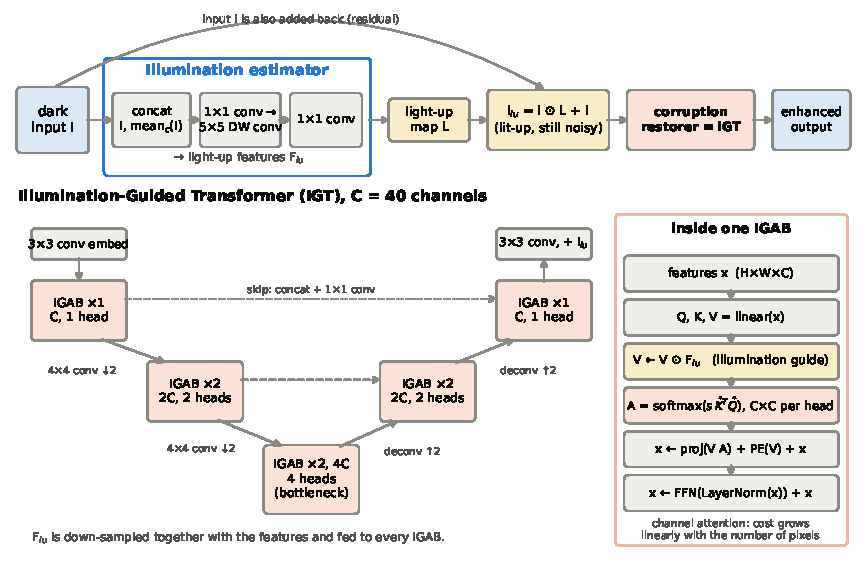
\includegraphics[width=0.86\textwidth]{architecture.pdf}
\caption{Retinexformer as implemented in the released code (our own drawing). Top: one-stage Retinex framework.
Bottom: the Illumination-Guided Transformer used as corruption restorer; right: operations inside one IGAB.}
\label{fig:arch}
\end{figure*}

\subsection{Proposed Noise-Aware Loss}
Retinexformer guides attention by illumination, but a dark pixel is not necessarily a noisy one, and the $\ell_1$
loss treats every pixel equally. We therefore weight the loss by an SNR map computed from the input, following the
estimator of SNR-Aware~\cite{xu2022snr}. With $g=\frac13\sum_c I_c$ the gray image and $\mathcal{B}_5$ a $5\times5$
mean filter,
\begin{equation}
b=\mathcal{B}_5(g),\quad n=|g-b|,\quad S=\frac{b}{n+\epsilon}, \label{eq:snr}
\end{equation}
with $\epsilon=10^{-4}$: $b$ estimates the local signal, $n$ the noise, and $S$ is large in clean, bright regions and
small in dark or noisy ones. The map is computed without gradients. Each pixel's SNR is converted to its rank within
the image, $r\in[0,1]$, and turned into a weight
\begin{equation}
w = 1+\alpha\,(1-r),\qquad \bar{w}=w\,/\,\mathrm{mean}(w), \label{eq:weight}
\end{equation}
so that the lowest-SNR pixel weighs $(1+\alpha)$ times as much as the highest-SNR pixel and the average weight is
exactly one. The SNR-weighted loss between output $\hat{Y}$ and ground truth $Y$ is
\begin{equation}
\mathcal{L}_{\mathrm{SNR}}=\frac{1}{3HW}\sum_{p,c}\bar{w}_p\,\bigl|\hat{Y}_{p,c}-Y_{p,c}\bigr|. \label{eq:lsnr}
\end{equation}

\emph{Two design decisions.} Both were made after measuring the SNR maps of LOL-v1 training images
(Fig.~\ref{fig:snr}). First, raw SNR values have an extreme tail; with min--max normalization, as initially planned,
93\% of the pixels of the example image receive a weight above 1.9, so the ``weighted'' loss would be nearly twice the
$\ell_1$ loss everywhere. That is a disguised doubling of the learning rate, not a re-weighting, and it would confound
the comparison with the control. Rank normalization spreads the weights evenly. Second, dividing by the mean keeps
the loss at the same scale as $\ell_1$, so only the \emph{distribution} of emphasis changes.

\begin{figure*}[t]
\centering
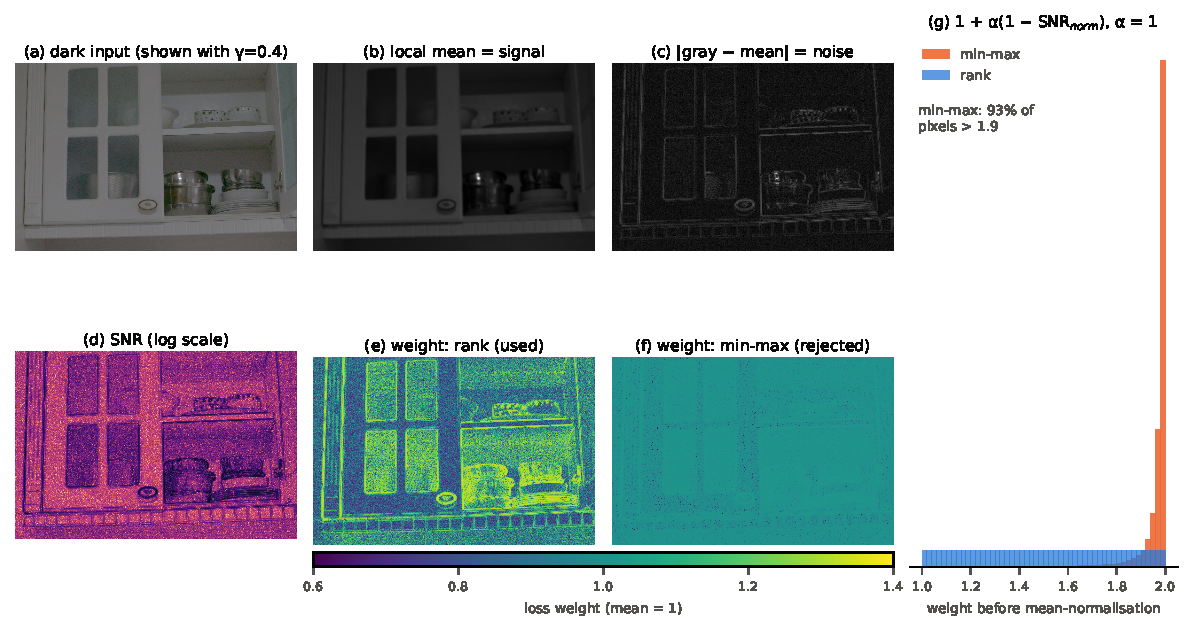
\includegraphics[width=0.92\textwidth]{snr_weights.pdf}
\caption{SNR-weighted loss on LOL-v1 test image 79, computed with the training code. (a) Input (display only).
(b) Local mean. (c) Noise estimate. (d) SNR (log scale). (e) Loss weights with rank normalization (used).
(f) With min--max normalization (rejected). (g) Weight distributions before mean-normalization: min--max puts 93\% of
pixels above 1.9.}
\label{fig:snr}
\end{figure*}

\subsection{Frequency-Domain Loss (Ablation)}
As a second variant we add a loss on Fourier amplitudes, which reflect global structure and colour distribution:
\begin{equation}
\mathcal{L}_{\mathrm{FFT}}=\mathrm{mean}\,\bigl|\,|\mathcal{F}(\hat{Y})|-|\mathcal{F}(Y)|\,\bigr|, \label{eq:fft}
\end{equation}
with $\mathcal{F}$ the orthonormal 2-D real FFT, used as $\mathcal{L}_1+\lambda\mathcal{L}_{\mathrm{FFT}}$ or
$\mathcal{L}_{\mathrm{SNR}}+\lambda\mathcal{L}_{\mathrm{FFT}}$ with $\lambda=0.05$.

\subsection{Detection-Based Evaluation}
To ask whether enhancement helps a machine, we run a COCO-pretrained YOLOv8m detector~\cite{jocher2023yolov8,lin2014coco}
\emph{without} re-training on the raw and on the enhanced versions of the same ExDark images. ExDark's twelve classes
are mapped to COCO categories (e.g. People$\rightarrow$person, Motorbike$\rightarrow$motorcycle, Table$\rightarrow$dining
table), predictions of the other 68 COCO classes are ignored, and boxes are converted from pixel coordinates to the
YOLO format. Because enhancement does not move objects, the labels are identical for all inputs.

% =====================================================================================================
\section{Experimental Setup}\label{sec:setup}
\subsection{Datasets}
Table~\ref{tab:data} lists the data. LOL-v1~\cite{wei2018retinexnet} and LOL-v2~\cite{yang2021lolv2} contain
low/normal-light pairs; LIME, DICM and MEF are unpaired real photos used for no-reference evaluation; ExDark~\cite{loh2019exdark}
provides box annotations. From the official ExDark test split we draw 100 images per class with a fixed seed
(1,200 images, 3,776 boxes, longer side at most 1,024~px), and a fixed 200-image subset of these for the slow
diffusion model. Labels were checked visually on sample images.

\emph{Overlap.} Comparing thumbnails, 91 of the 100 LOL-v2-real test images are identical to LOL-v1 training images.
Any model trained on LOL-v1 is therefore not evaluated on LOL-v2-real in this report.

\begin{table}[t]
\centering
\caption{Datasets used}
\label{tab:data}
\begin{tabular}{l l r r}
\toprule
Dataset & Type & Train & Test \\
\midrule
LOL-v1 & paired, real & 485 & 15 \\
LOL-v2-real & paired, real & 689 & 100 \\
LOL-v2-syn & paired, synthetic & 900 & 100 \\
LIME / DICM / MEF & unpaired, real & -- & 10 / 69 / 17 \\
ExDark (our subset) & detection, 12 classes & -- & 1,200 \\
\bottomrule
\end{tabular}
\end{table}

\subsection{Metrics}
PSNR measures pixel fidelity, $\mathrm{PSNR}=10\log_{10}\bigl(1/\mathrm{MSE}(\hat{Y},Y)\bigr)$ for images in $[0,1]$;
SSIM~\cite{wang2004ssim} compares local luminance, contrast and structure; LPIPS~\cite{zhang2018lpips} is a distance
between deep features (AlexNet) that correlates better with human judgement; NIQE~\cite{mittal2013niqe} needs no
reference and measures the distance to natural-image statistics. \emph{Dark-region PSNR/SSIM} restrict the error to a
mask $M$ of the 30\% darkest pixels of the input (by luminance), $\mathrm{PSNR}_M=10\log_{10}(1/\mathrm{MSE}_M)$, to test
where noise is strongest. For detection we report mAP50 and mAP50-95 (box IoU thresholds 0.5 and 0.5--0.95),
precision and recall. Arrows in the tables show whether higher ($\uparrow$) or lower ($\downarrow$) is better.

\subsection{Baselines and Protocol}
HE, CLAHE and gamma correction ($\gamma=0.4$) operate on the lightness channel; Zero-DCE, SCI, LLFormer, GSAD and
Retinexformer use their official weights (LOL-v1 weights for LLFormer and for Retinexformer on unpaired data);
SNR-Aware is evaluated on the output images released by its authors. All outputs are scored by the same
evaluation script. Three rules apply throughout: (i) no ground-truth information at test time---GSAD is reported on
its raw output, and its ground-truth-brightness-corrected output only for comparison with its paper; (ii) no
checkpoint is chosen by its test score; (iii) no model is evaluated on test images it was trained on.

\subsection{Implementation Details}
Training ran on Kaggle Tesla T4 GPUs (PyTorch 2.11); evaluation ran on a laptop (PyTorch 2.14). Two pitfalls of the
laptop GPU (Apple MPS) were found by direct comparison with the CPU: it produces wrong outputs for LLFormer and
wrong YOLOv8 scores (mAP50 0.42 vs.\ 0.65 on the same 100 images), so these run on the CPU, and all timings come from
one T4.

\emph{Re-training.} Retinexformer was trained from scratch on LOL-v1 with the official configuration (150k iterations,
batch 8, $128\times128$ patches, Adam, cosine schedule) in two Kaggle sessions (about 11.9 GPU hours, 0.28 s/iteration).

\emph{Fine-tuning experiment.} Four runs start from the released LOL-v1 weights and differ only in the loss:
A $\mathcal{L}_1$ (control), B $\mathcal{L}_{\mathrm{SNR}}$, C $\mathcal{L}_1+\lambda\mathcal{L}_{\mathrm{FFT}}$,
D $\mathcal{L}_{\mathrm{SNR}}+\lambda\mathcal{L}_{\mathrm{FFT}}$. All use 10,000 iterations, batch 8, $128\times128$
random crops with horizontal/vertical flips from the LOL-v1 training set, Adam with a cosine decay from
$2\times10^{-5}$ to $10^{-6}$, gradient-norm clipping at 0.01, $\alpha=1$, $\lambda=0.05$, and seed 42. The whole
sequence of batches is pre-computed from the seed, so every run sees exactly the same crops in the same order; the
final weights are evaluated.

% =====================================================================================================
\section{Results}\label{sec:results}
\subsection{Quantitative Comparison}
Table~\ref{tab:main} compares all methods on the paired test sets. Retinexformer has the highest PSNR on all three
sets. GSAD, evaluated without the ground-truth correction, has the lowest LPIPS everywhere and the highest SSIM on
LOL-v1, but a lower PSNR. Classical and zero-shot methods brighten the image but stay far below the supervised
transformers, and CLAHE improves the input only slightly because it redistributes contrast without raising the
overall brightness enough.

\begin{table*}[t]
\centering
\caption{Quantitative comparison on paired test sets (best in bold). $^{\dagger}$Output images released by the
authors. ``--'': not evaluated because of train/test overlap or because only LOL-v1 weights exist.}
\label{tab:main}
\begin{tabular}{l ccc ccc ccc}
\toprule
 & \multicolumn{3}{c}{LOL-v1} & \multicolumn{3}{c}{LOL-v2-real} & \multicolumn{3}{c}{LOL-v2-syn} \\
\cmidrule(lr){2-4}\cmidrule(lr){5-7}\cmidrule(lr){8-10}
Method & PSNR$\uparrow$ & SSIM$\uparrow$ & LPIPS$\downarrow$ & PSNR$\uparrow$ & SSIM$\uparrow$ & LPIPS$\downarrow$ & PSNR$\uparrow$ & SSIM$\uparrow$ & LPIPS$\downarrow$ \\
\midrule
Input (no enhancement) & 7.77 & 0.191 & 0.560 & 9.72 & 0.196 & 0.519 & 11.22 & 0.450 & 0.379 \\
HE & 14.26 & 0.425 & 0.602 & 13.48 & 0.435 & 0.551 & 15.63 & 0.728 & 0.310 \\
CLAHE & 9.13 & 0.356 & 0.503 & 11.54 & 0.420 & 0.424 & 12.45 & 0.556 & 0.360 \\
Gamma ($\gamma{=}0.4$) & 14.53 & 0.620 & 0.351 & 18.70 & 0.659 & 0.318 & 18.11 & 0.827 & 0.183 \\
\midrule
Zero-DCE~\cite{guo2020zerodce} & 14.86 & 0.562 & 0.335 & 18.06 & 0.580 & 0.313 & 17.76 & 0.814 & 0.168 \\
SCI~\cite{ma2022sci} & 14.85 & 0.527 & 0.339 & 17.36 & 0.542 & 0.307 & 15.43 & 0.747 & 0.233 \\
\midrule
SNR-Aware$^{\dagger}$~\cite{xu2022snr} & 24.61 & 0.840 & 0.151 & 21.48 & \textbf{0.848} & 0.157 & 24.14 & 0.927 & 0.056 \\
LLFormer~\cite{wang2023llformer} & 23.65 & 0.816 & 0.169 & -- & -- & -- & -- & -- & -- \\
GSAD~\cite{hou2023gsad} & 22.73 & \textbf{0.850} & \textbf{0.103} & 20.14 & 0.845 & \textbf{0.114} & 24.10 & 0.927 & \textbf{0.052} \\
Retinexformer~\cite{cai2023retinexformer} & \textbf{25.15} & 0.843 & 0.131 & \textbf{22.79} & 0.839 & 0.171 & \textbf{25.67} & \textbf{0.928} & 0.059 \\
Retinexformer (our re-training) & 23.10 & 0.828 & 0.143 & -- & -- & -- & -- & -- & -- \\
\bottomrule
\end{tabular}

\end{table*}


\subsection{Reproduction of Published Results}
Table~\ref{tab:repro} compares our numbers with those reported in the original papers under the same protocol.
Retinexformer, SNR-Aware and LLFormer are reproduced to within 0.01~dB. GSAD's reported numbers are obtained after
rescaling each output so that its mean gray level equals that of the ground truth; reproducing that protocol, we
are within 0.14--0.43~dB of the paper, but the correction is worth 4.8, 8.5 and 4.1~dB on the three sets (27.57 vs.\
22.73~dB on LOL-v1), which is more than the gap between most published methods.

\begin{table}[t]
\centering
\caption{Our results vs.\ numbers reported in the original papers}
\label{tab:repro}
\resizebox{\columnwidth}{!}{\begin{tabular}{ll cc cc r}
\toprule
 & & \multicolumn{2}{c}{Reported} & \multicolumn{2}{c}{Ours} & \\
\cmidrule(lr){3-4}\cmidrule(lr){5-6}
Method & Set & PSNR & SSIM & PSNR & SSIM & $\Delta$PSNR \\
\midrule
Retinexformer & LOL-v1 & 25.16 & 0.845 & 25.15 & 0.843 & -0.01 \\
Retinexformer & LOL-v2-real & 22.80 & 0.840 & 22.79 & 0.839 & -0.01 \\
Retinexformer & LOL-v2-syn & 25.67 & 0.930 & 25.67 & 0.928 & 0.00 \\
SNR-Aware$^{\dagger}$ & LOL-v1 & 24.61 & 0.842 & 24.61 & 0.840 & 0.00 \\
SNR-Aware$^{\dagger}$ & LOL-v2-real & 21.48 & 0.849 & 21.48 & 0.848 & 0.00 \\
SNR-Aware$^{\dagger}$ & LOL-v2-syn & 24.14 & 0.928 & 24.14 & 0.927 & 0.00 \\
LLFormer & LOL-v1 & 23.65 & 0.816 & 23.65 & 0.816 & 0.00 \\
GSAD$^{\ddagger}$ & LOL-v1 & 27.84 & 0.877 & 27.57 & 0.875 & -0.27 \\
GSAD$^{\ddagger}$ & LOL-v2-real & 28.82 & 0.895 & 28.68 & 0.893 & -0.14 \\
GSAD$^{\ddagger}$ & LOL-v2-syn & 28.67 & 0.944 & 28.24 & 0.942 & -0.43 \\
\bottomrule
\end{tabular}
}\\[2pt]
\footnotesize $^{\dagger}$Authors' released images. $^{\ddagger}$Both rows use GSAD's ground-truth brightness correction.
\end{table}

\emph{Re-training Retinexformer.} Training from scratch with the official configuration gives 23.10~dB / 0.828 SSIM on
LOL-v1 with the final model, against 25.15~dB for the released weights (Fig.~\ref{fig:train}). The best validation
value during training, 23.61~dB at 94k iterations, was measured on the test images, so it is not used as a result.
Our evaluation script reproduces the training-time validation PSNR exactly, so the gap is not a metric difference.
An independent attempt reported on the authors' repository reached 23.45~dB. Likely causes are run-to-run variance
on a dataset with only 485 training and 15 test images, a different software and hardware stack, and the possibility
that the released checkpoint was selected among several; validation PSNR had plateaued from about 110k iterations.

\begin{figure}[t]
\centering
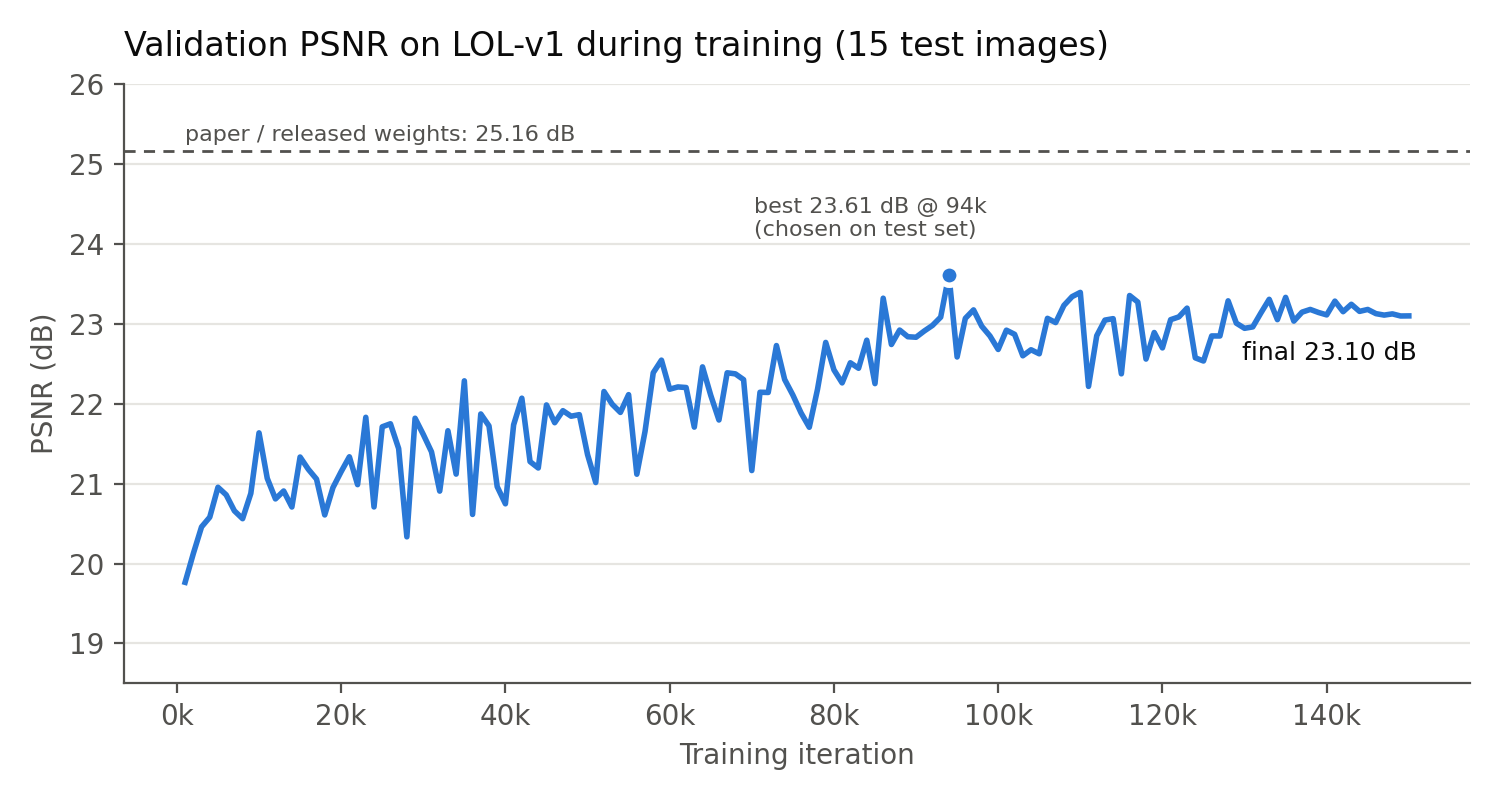
\includegraphics[width=\columnwidth]{training_val_psnr.png}
\caption{Validation PSNR on LOL-v1 while re-training Retinexformer from scratch (150k iterations).}
\label{fig:train}
\end{figure}

\subsection{No-Reference Evaluation}
Table~\ref{tab:noref} gives NIQE on the unpaired sets. No method is best everywhere: Zero-DCE has the lowest NIQE on
LIME and MEF and Retinexformer on DICM. NIQE measures naturalness, not fidelity, and methods trained on LOL do not
automatically produce the most natural-looking results on other cameras.

\begin{table}[t]
\centering
\caption{NIQE ($\downarrow$) on unpaired real photos}
\label{tab:noref}
\begin{tabular}{l ccc}
\toprule
Method & LIME & DICM & MEF \\
\midrule
Input (no enhancement) & 4.351 & 4.273 & 4.266 \\
HE & 3.878 & 3.800 & 3.931 \\
CLAHE & 3.912 & 3.792 & 3.605 \\
Gamma ($\gamma{=}0.4$) & 3.906 & 3.900 & 3.383 \\
Zero-DCE~\cite{guo2020zerodce} & \textbf{3.771} & 3.742 & \textbf{3.283} \\
SCI~\cite{ma2022sci} & 4.202 & 4.139 & 3.638 \\
Retinexformer~\cite{cai2023retinexformer} & 4.074 & \textbf{3.421} & 3.438 \\
Retinexformer (our re-training) & 3.944 & 3.591 & 3.512 \\
\bottomrule
\end{tabular}

\end{table}

\subsection{Qualitative Comparison}
Fig.~\ref{fig:grid} shows LOL-v1 results with zoomed crops of dark regions. The zero-shot methods brighten the
scene but leave strong colour noise in the dark areas; the supervised transformers remove it but blur fine texture;
GSAD keeps the most texture but shifts colours (green cast on image 493). Unpaired examples are shown in
Fig.~\ref{fig:lime}.

\begin{figure*}[t]
\centering
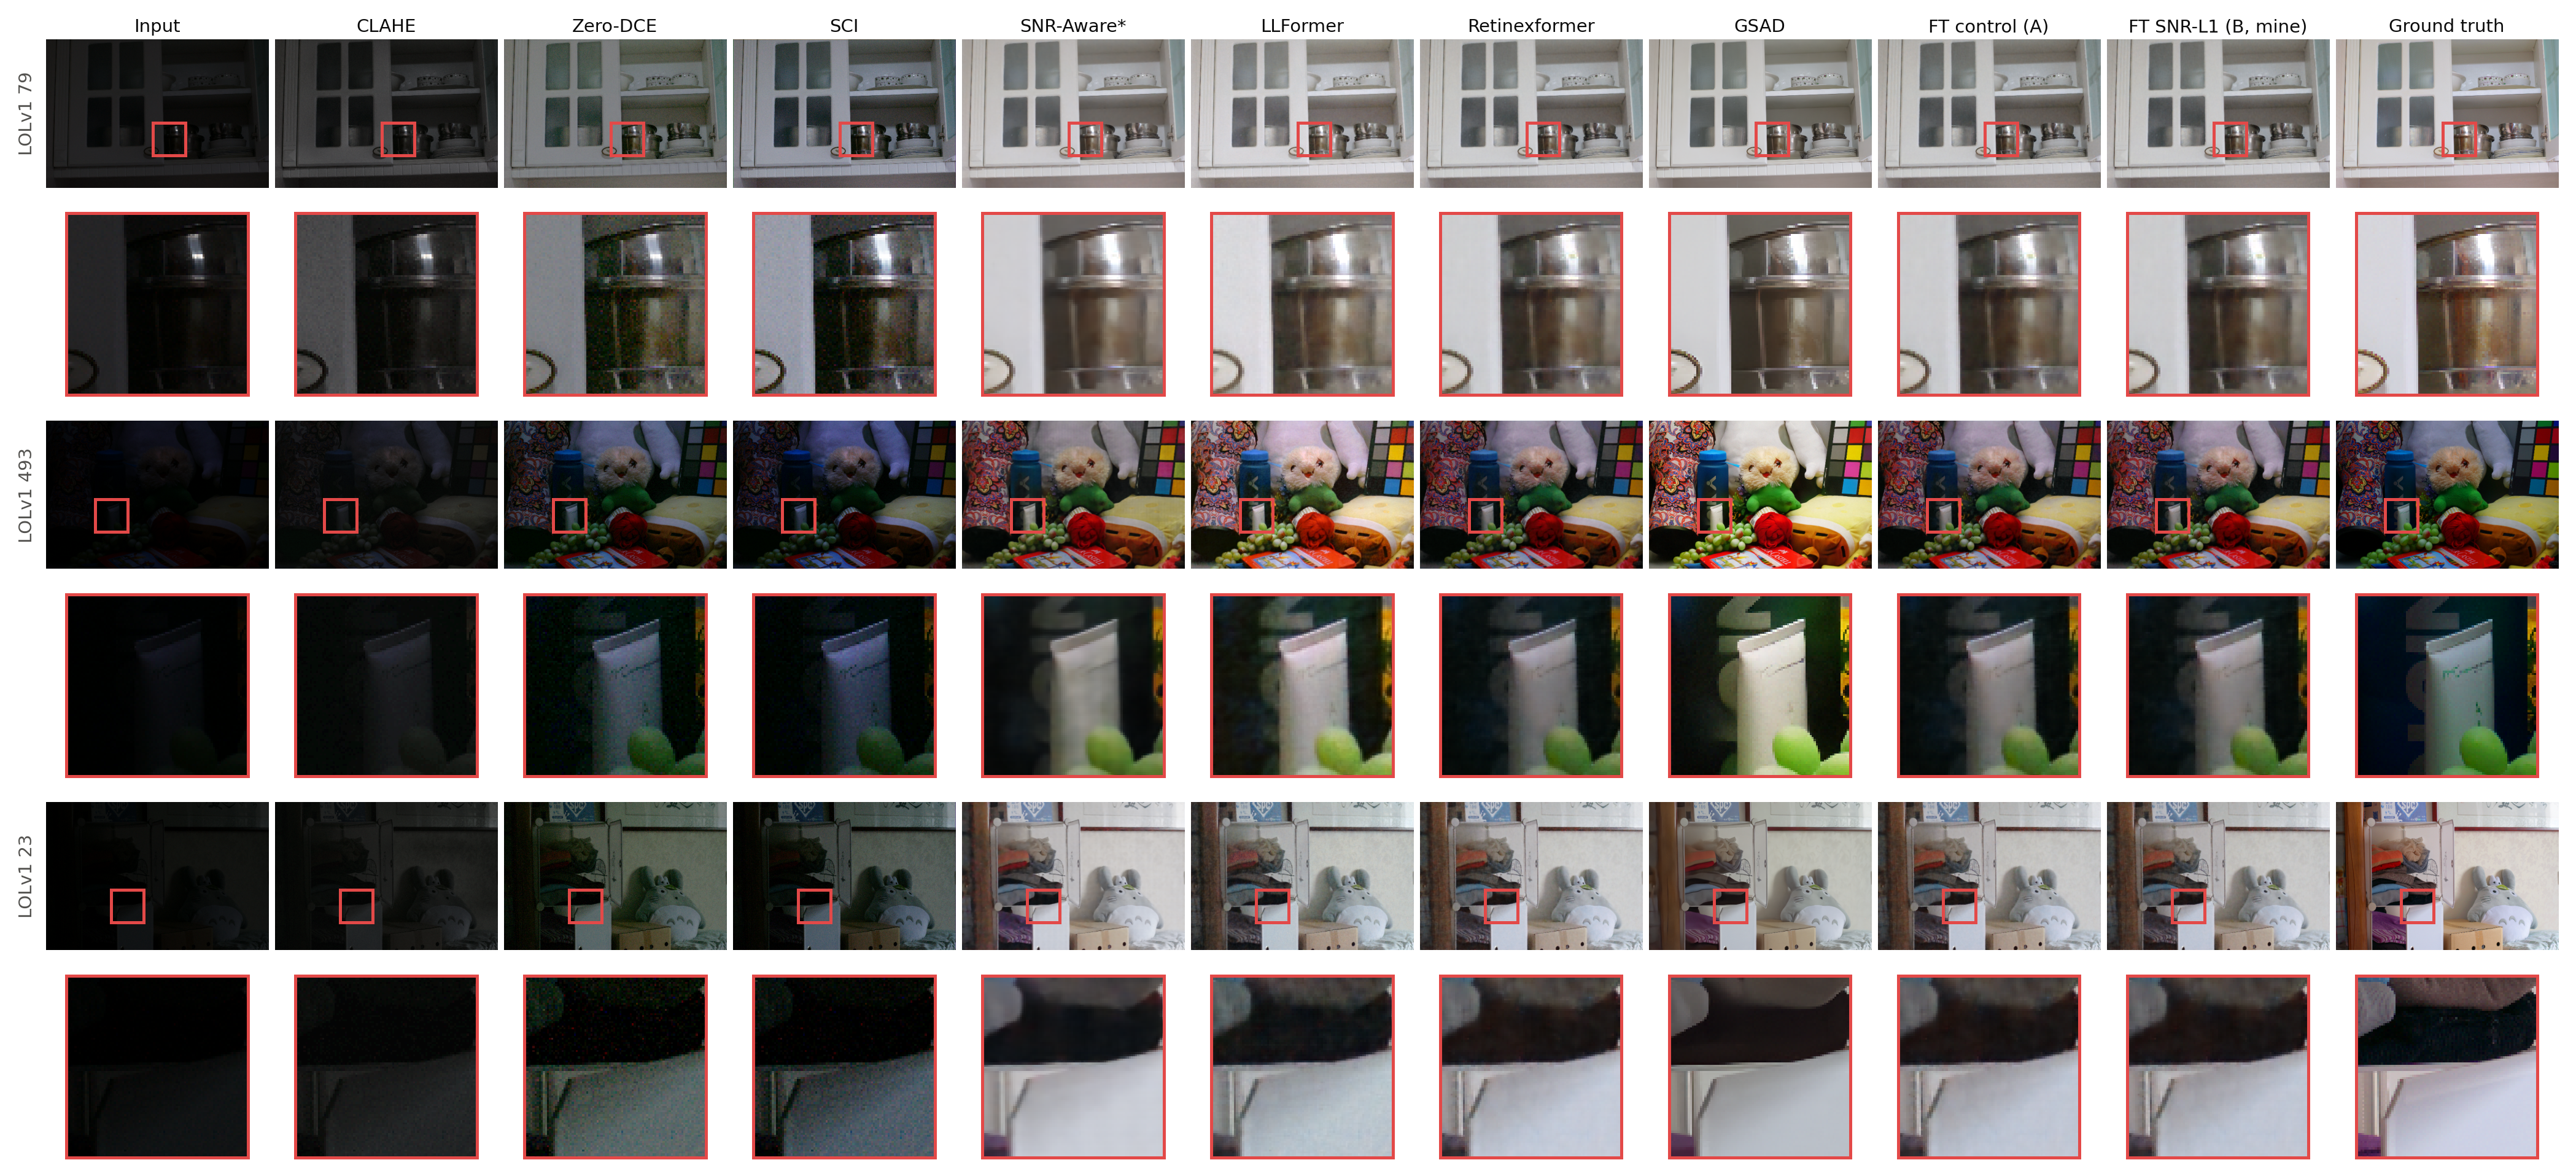
\includegraphics[width=\textwidth]{grid_lolv1.png}
\caption{Qualitative comparison on LOL-v1. Red boxes mark a region that is dark in the input but detailed in the
ground truth; the enlarged crops are shown below each image. $^{*}$Released images. FT: fine-tuned runs A and B.}
\label{fig:grid}
\end{figure*}

\begin{figure}[t]
\centering
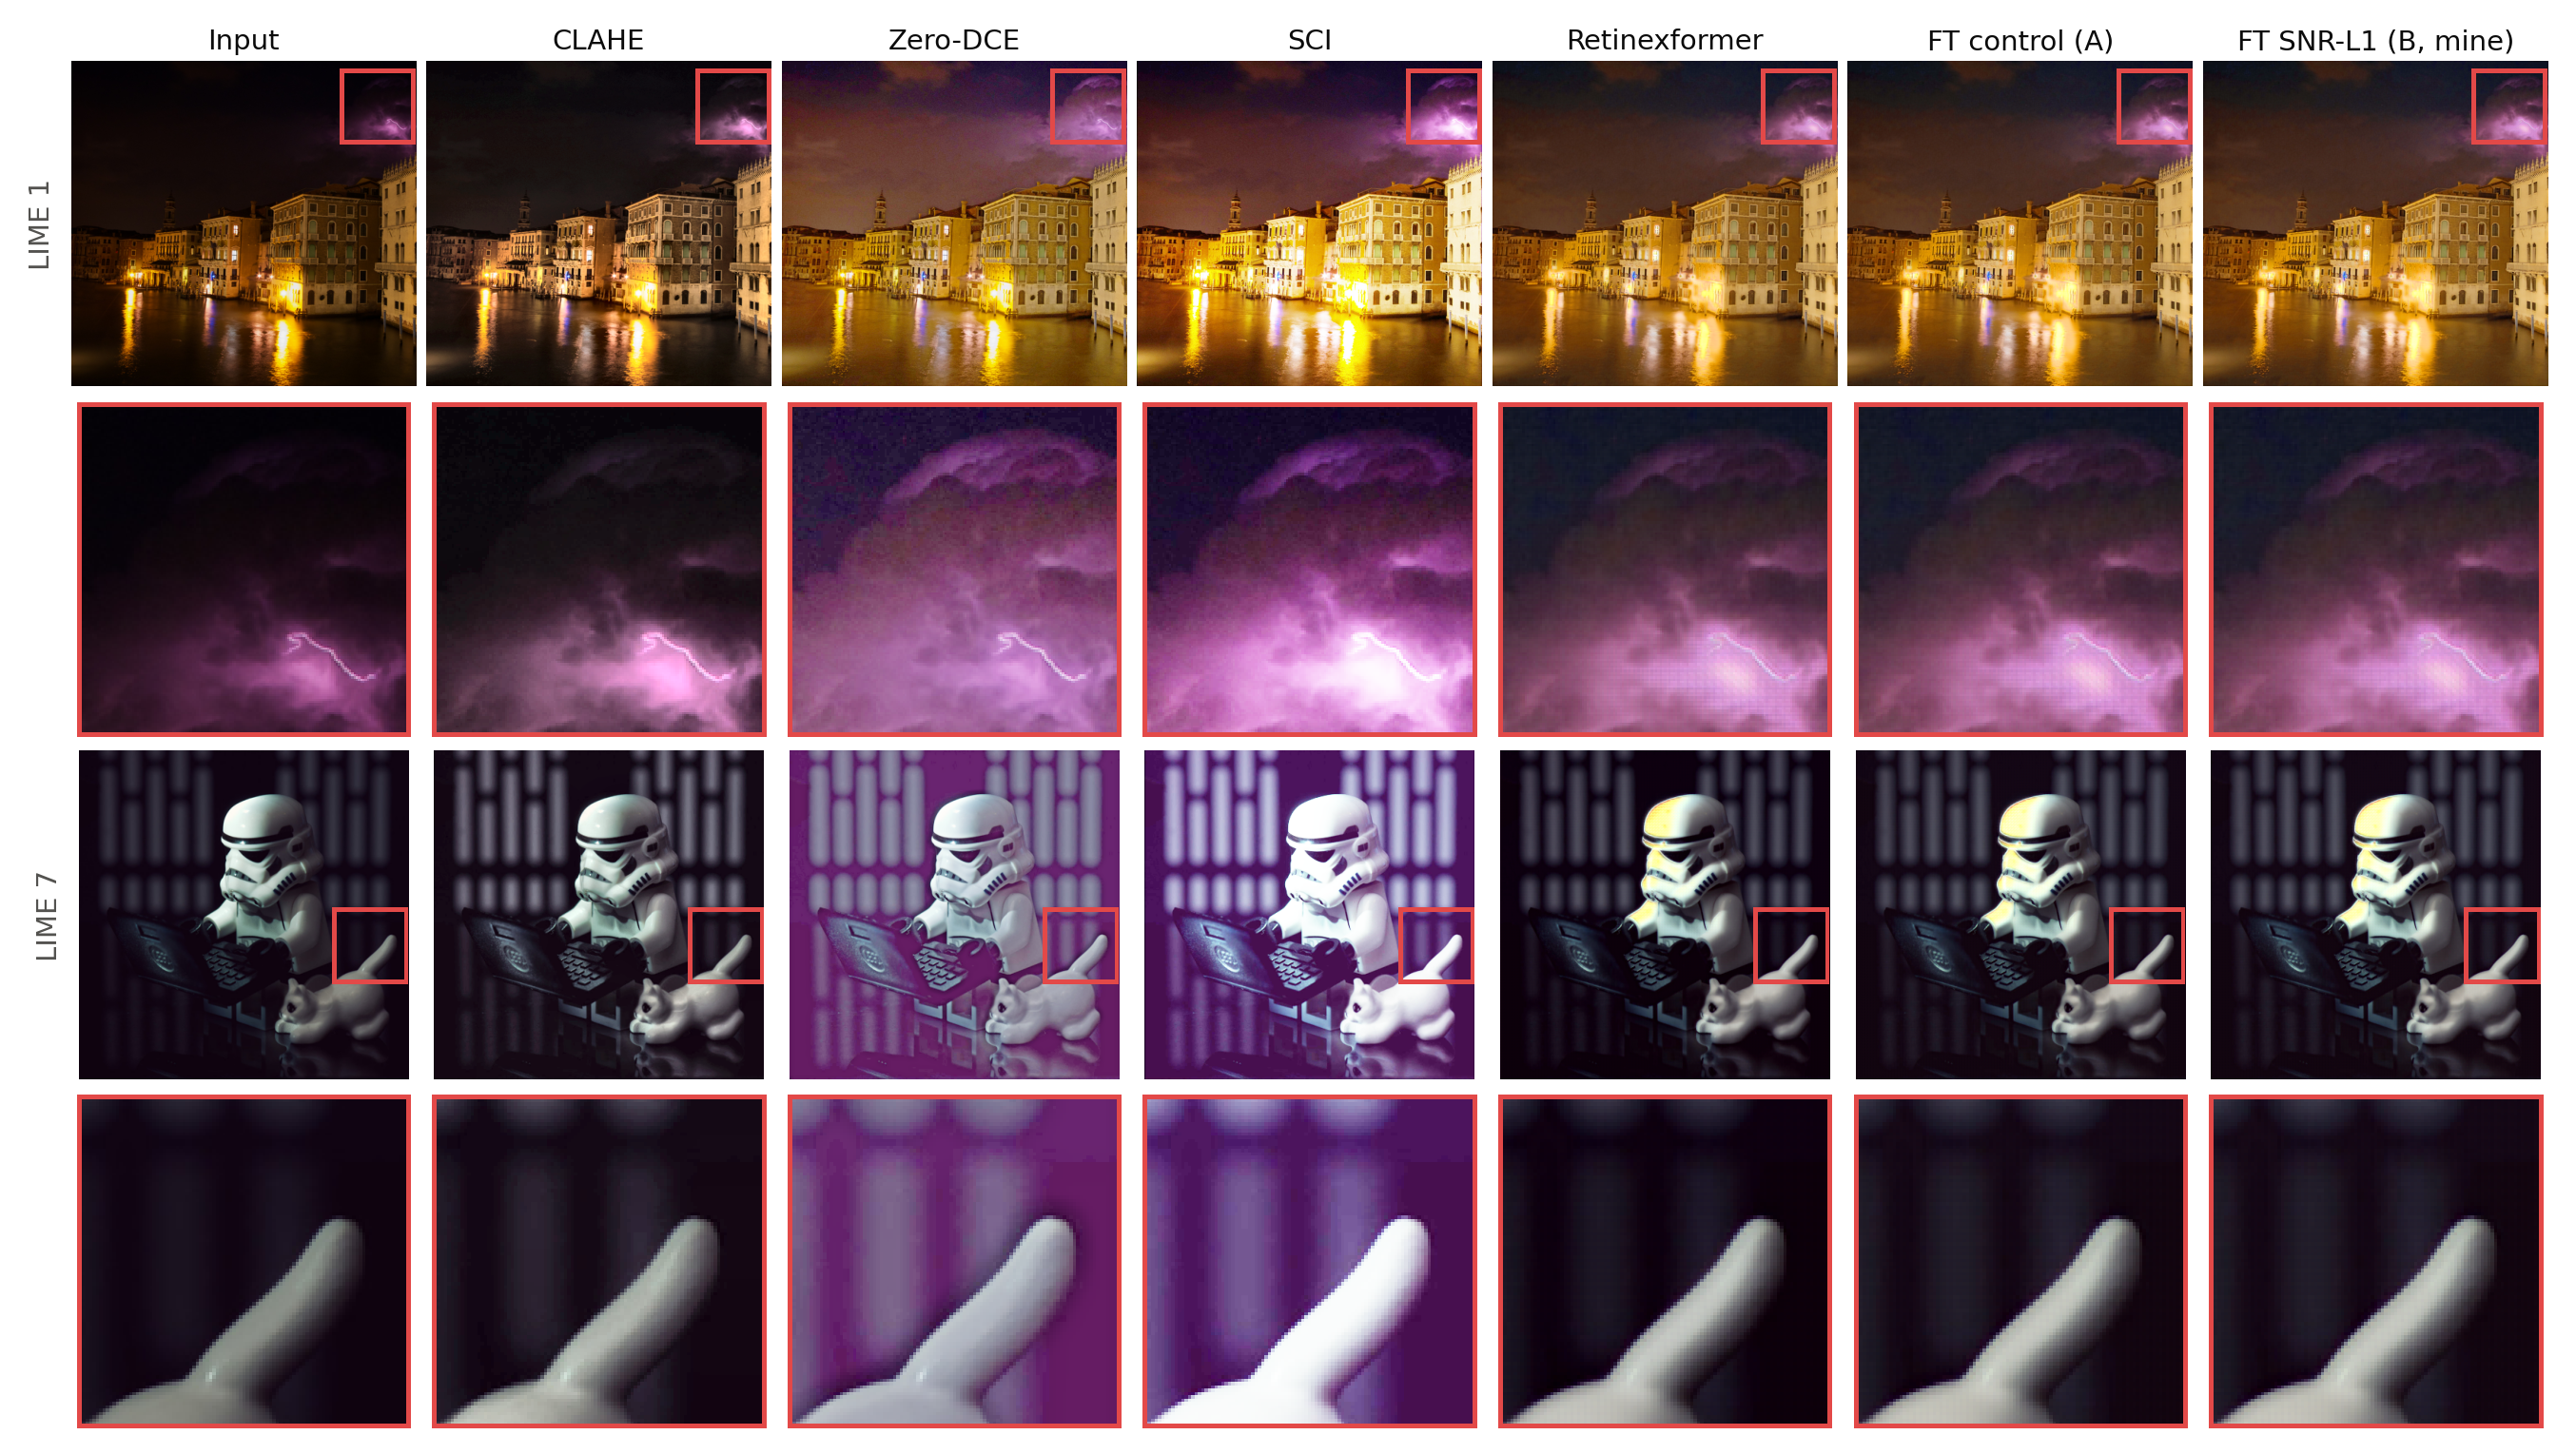
\includegraphics[width=\columnwidth]{grid_lime.png}
\caption{Unpaired LIME images (no ground truth). Zoomed crops: dark regions of the input.}
\label{fig:lime}
\end{figure}

\begin{table*}[t]
\centering
\caption{Controlled fine-tuning experiment (only the loss differs between A--D). Wins: number of LOL-v1 test images on
which a run beats the control A, over the whole image and in the darkest 30\% of pixels. NIQE: mean over LIME, DICM,
MEF. ExDark-200 rows were all computed on one T4.}
\label{tab:abl}
\begin{tabular}{l ccc c cc c c c}
\toprule
 & \multicolumn{3}{c}{LOL-v1} & Dark 30\% & \multicolumn{2}{c}{Wins vs.\ A} & LOL-v2-syn & NIQE & ExDark-200 \\
\cmidrule(lr){2-4}\cmidrule(lr){6-7}
Run & PSNR$\uparrow$ & SSIM$\uparrow$ & LPIPS$\downarrow$ & PSNR$\uparrow$ & image & dark & PSNR$\uparrow$ & mean$\downarrow$ & mAP50$\uparrow$ \\
\midrule
Released (start point) & \textbf{25.15} & \textbf{0.843} & \textbf{0.131} & \textbf{25.31} & -- & -- & 16.19 & \textbf{3.644} & \textbf{0.627} \\
\midrule
A: $\mathcal{L}_1$ (control) & 24.31 & 0.842 & 0.132 & 24.89 & -- & -- & 16.61 & \textbf{3.644} & \textbf{0.627} \\
B: $\mathcal{L}_{\mathrm{SNR}}$ (ours) & 24.32 & 0.842 & \textbf{0.131} & 24.91 & 11/15 & 13/15 & \textbf{16.62} & 3.704 & 0.626 \\
C: $\mathcal{L}_1{+}\lambda\mathcal{L}_{\mathrm{FFT}}$ & 24.31 & 0.842 & \textbf{0.131} & 24.89 & 8/15 & 3/15 & 16.61 & \textbf{3.644} & 0.626 \\
D: $\mathcal{L}_{\mathrm{SNR}}{+}\lambda\mathcal{L}_{\mathrm{FFT}}$ & 24.32 & 0.842 & \textbf{0.131} & 24.91 & 10/15 & 12/15 & \textbf{16.62} & 3.696 & 0.626 \\
\bottomrule
\end{tabular}

\end{table*}

\subsection{Detection on ExDark}
Table~\ref{tab:det} shows that every enhancer lowers the mAP of the pretrained detector. On 1,200 images mAP50 falls
from 0.662 on raw images to 0.603 (Retinexformer), 0.595 (SCI) and 0.572 (Zero-DCE); on the 200-image subset the
diffusion model is the best enhancer (0.633) but still below raw images (0.707). The loss is almost entirely in
recall, while precision is roughly unchanged: after enhancement the detector misses objects rather than inventing
them. Among enhancers the ranking follows image quality, so better restoration hurts less, but none helps. Examples are
shown in Fig.~\ref{fig:det}: a school bus is not detected in any version, and enhancement turns a white blanket
yellow.

\begin{table}[t]
\centering
\caption{YOLOv8m on ExDark: raw vs.\ enhanced inputs (best in bold)}
\label{tab:det}
\resizebox{\columnwidth}{!}{\begin{tabular}{l ccc ccc}
\toprule
 & \multicolumn{3}{c}{1{,}200 images} & \multicolumn{3}{c}{200-image subset} \\
\cmidrule(lr){2-4}\cmidrule(lr){5-7}
Input to YOLOv8m & mAP50 & mAP50-95 & Recall & mAP50 & mAP50-95 & Recall \\
\midrule
Raw (no enhancement) & \textbf{0.662} & \textbf{0.345} & \textbf{0.611} & \textbf{0.707} & \textbf{0.378} & \textbf{0.637} \\
Zero-DCE & 0.572 & 0.291 & 0.502 & 0.603 & 0.317 & 0.513 \\
SCI & 0.595 & 0.301 & 0.529 & 0.625 & 0.330 & 0.577 \\
Retinexformer & 0.603 & 0.310 & 0.540 & 0.628 & 0.340 & 0.553 \\
GSAD & -- & -- & -- & 0.633 & 0.342 & 0.560 \\
\bottomrule
\end{tabular}
}
\end{table}

\begin{figure}[t]
\centering
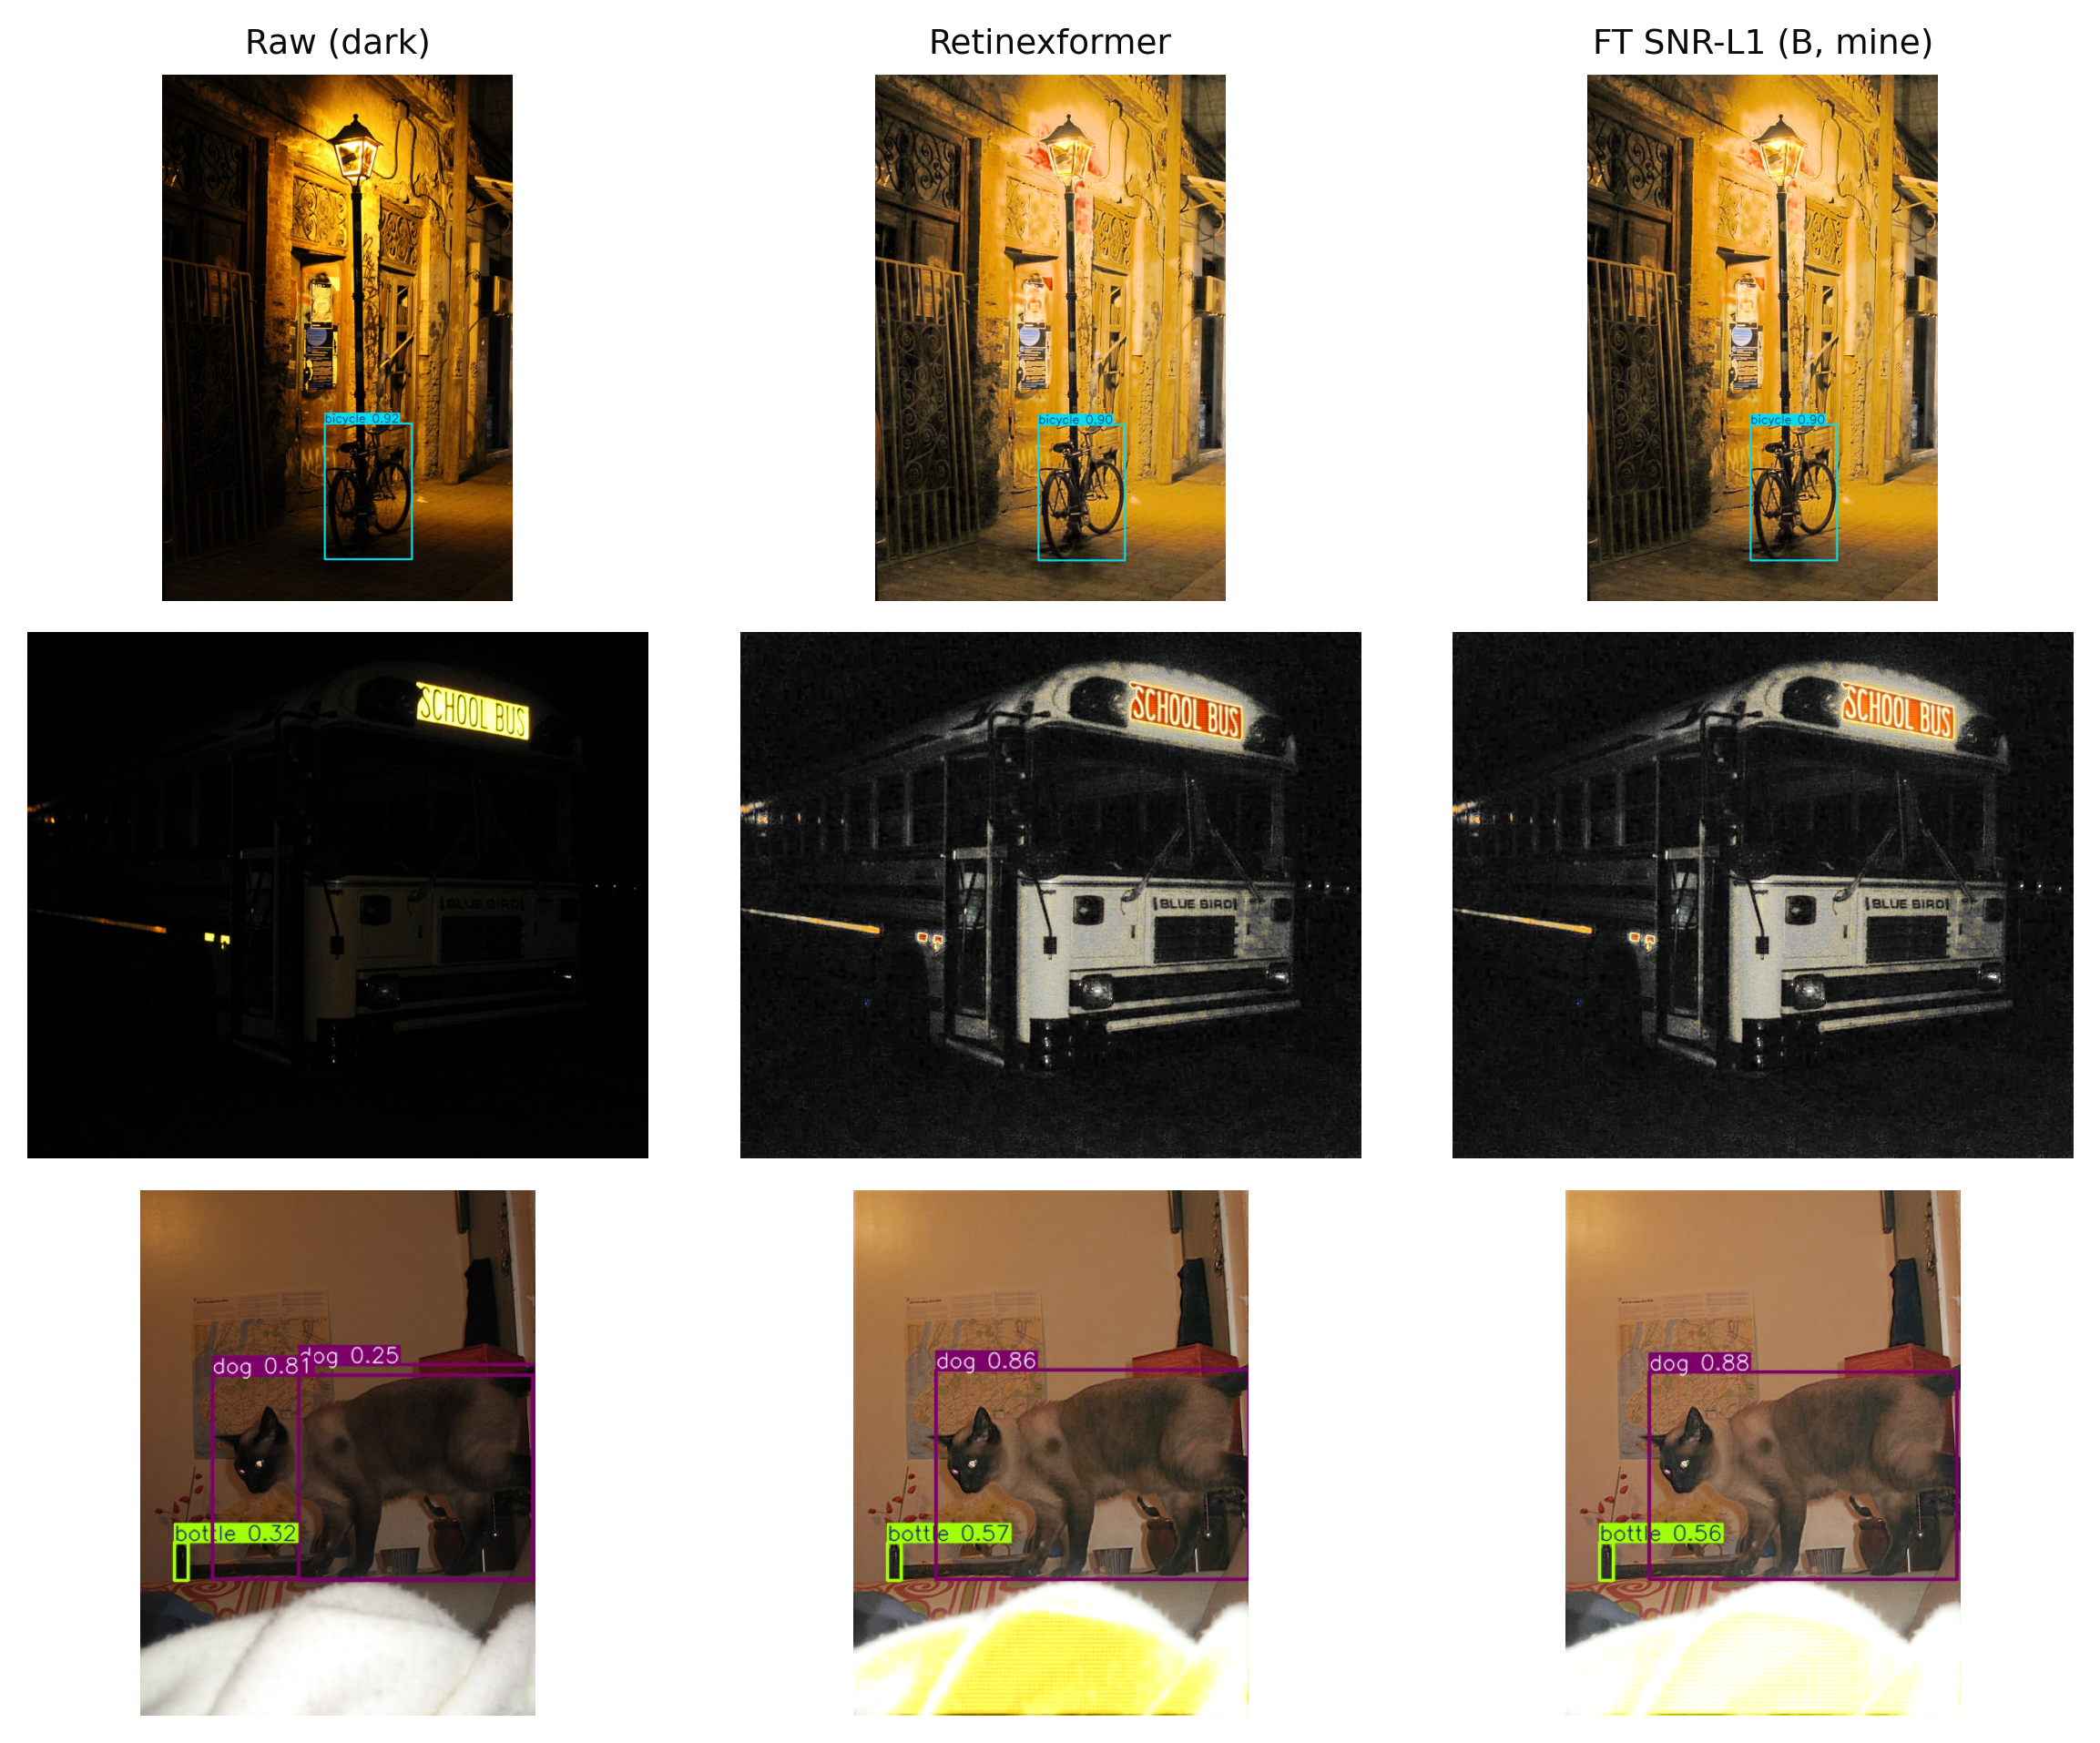
\includegraphics[width=\columnwidth]{detection_examples.png}
\caption{YOLOv8m detections (confidence $\geq0.25$) on raw and enhanced ExDark images.}
\label{fig:det}
\end{figure}

This does not contradict Retinexformer's own detection experiment, which trains YOLOv3 from scratch on enhanced
images and compares enhancers with each other; its table does not include a raw-input row. Our experiment answers a
different question: does enhancement help a detector that was trained on normal-light images?

\subsection{Efficiency}
Table~\ref{tab:eff} and Fig.~\ref{fig:speed} report parameters and network time per $600\times400$ image on one T4.
Retinexformer gives the best PSNR at 151~ms per image with 1.61~M parameters; GSAD needs 2.4--4.9~s per image
(10 or 20 sampling steps), 16--32 times slower, and LLFormer is about six times slower with fifteen times more
parameters.

\begin{table}[t]
\centering
\caption{Efficiency on one Tesla T4 ($600\times400$ input)}
\label{tab:eff}
\begin{tabular}{l rr}
\toprule
Method & Params (M) & Time (ms/img) \\
\midrule
SCI & 0.0003 & 1.5 \\
Zero-DCE & 0.0794 & 19.1 \\
Retinexformer & 1.61 & 151.3 \\
LLFormer & 24.55 & 874.4 \\
GSAD (10 steps) & 17.44 & 2,360.0 \\
GSAD (20 steps) & 17.44 & 4,873.6 \\
\bottomrule
\end{tabular}

\end{table}

\begin{figure}[t]
\centering
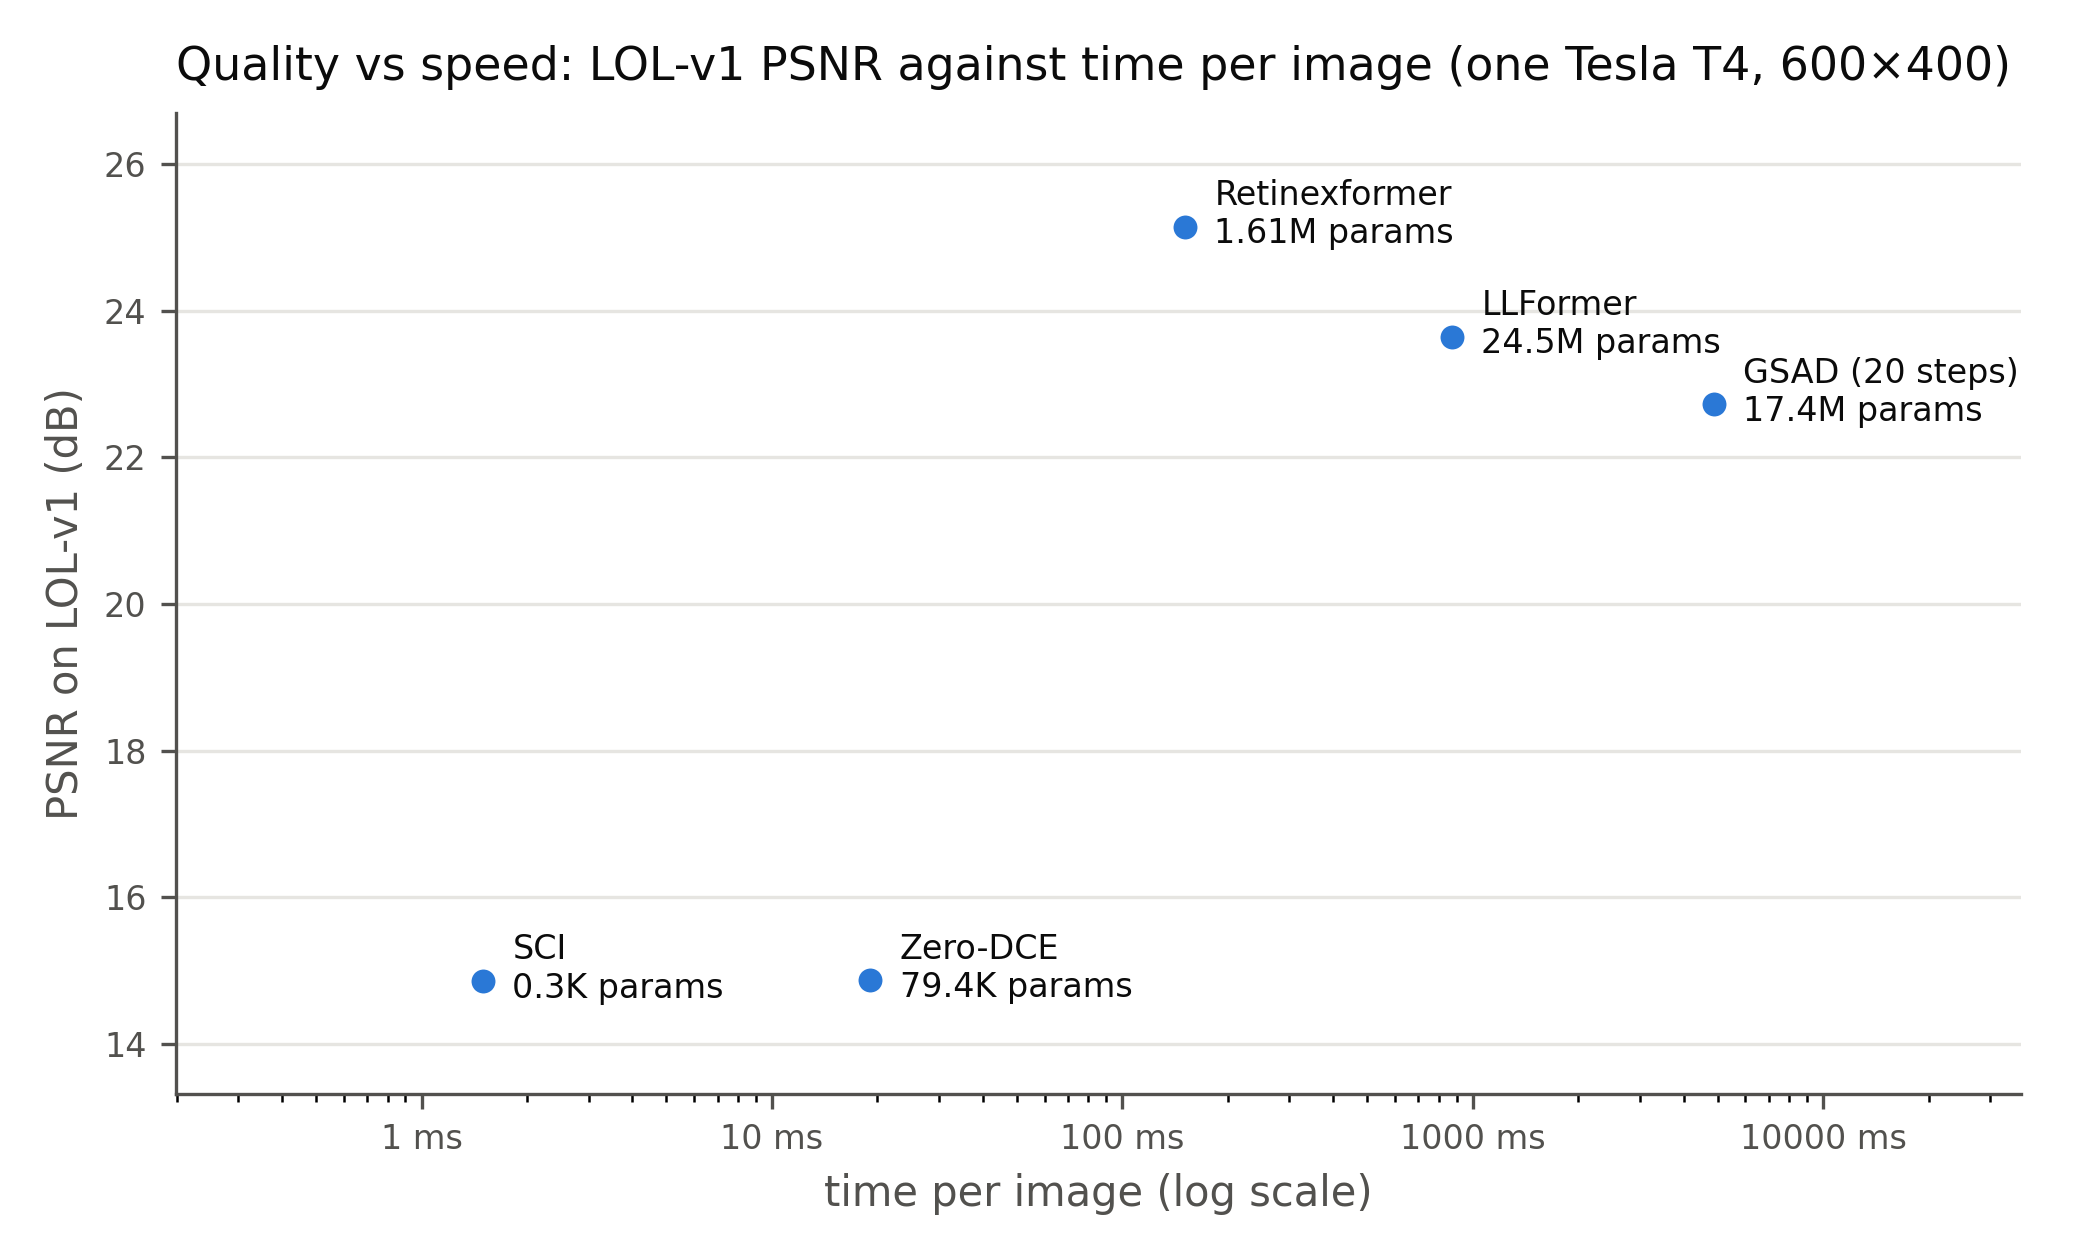
\includegraphics[width=\columnwidth]{quality_vs_speed.png}
\caption{LOL-v1 PSNR against time per image (log scale), one Tesla T4.}
\label{fig:speed}
\end{figure}

\subsection{Ablation: Noise-Aware Loss}
Table~\ref{tab:abl} gives the controlled experiment. All four runs reduce the training $\ell_1$ loss from 0.040 to 0.035
(Fig.~\ref{fig:ft}), and their curves overlap almost exactly. Fine-tuning itself lowers LOL-v1 PSNR from 25.15 to
24.31--24.32~dB in every run, including the control, while LOL-v2-syn PSNR rises from 16.19 to 16.61--16.62~dB.


Compared with the control, the SNR-weighted loss (B) changes PSNR by +0.01~dB overall and +0.02~dB in the darkest
regions. The direction is consistent: B beats A in the dark regions on 13 of 15 images (one-sided sign test
$p=0.004$), whereas over whole images it wins on 11 of 15 ($p=0.06$). The size of the effect, however, is far below
what is visible or what a 15-image test set can resolve in average PSNR. The FFT term (C) has no effect and is
slightly worse than A in dark regions (3 of 15 wins); combining both (D) behaves like B. NIQE is slightly worse for
the SNR loss on DICM, and detection is unchanged (0.626 vs.\ 0.627 mAP50).

\begin{figure}[t]
\centering
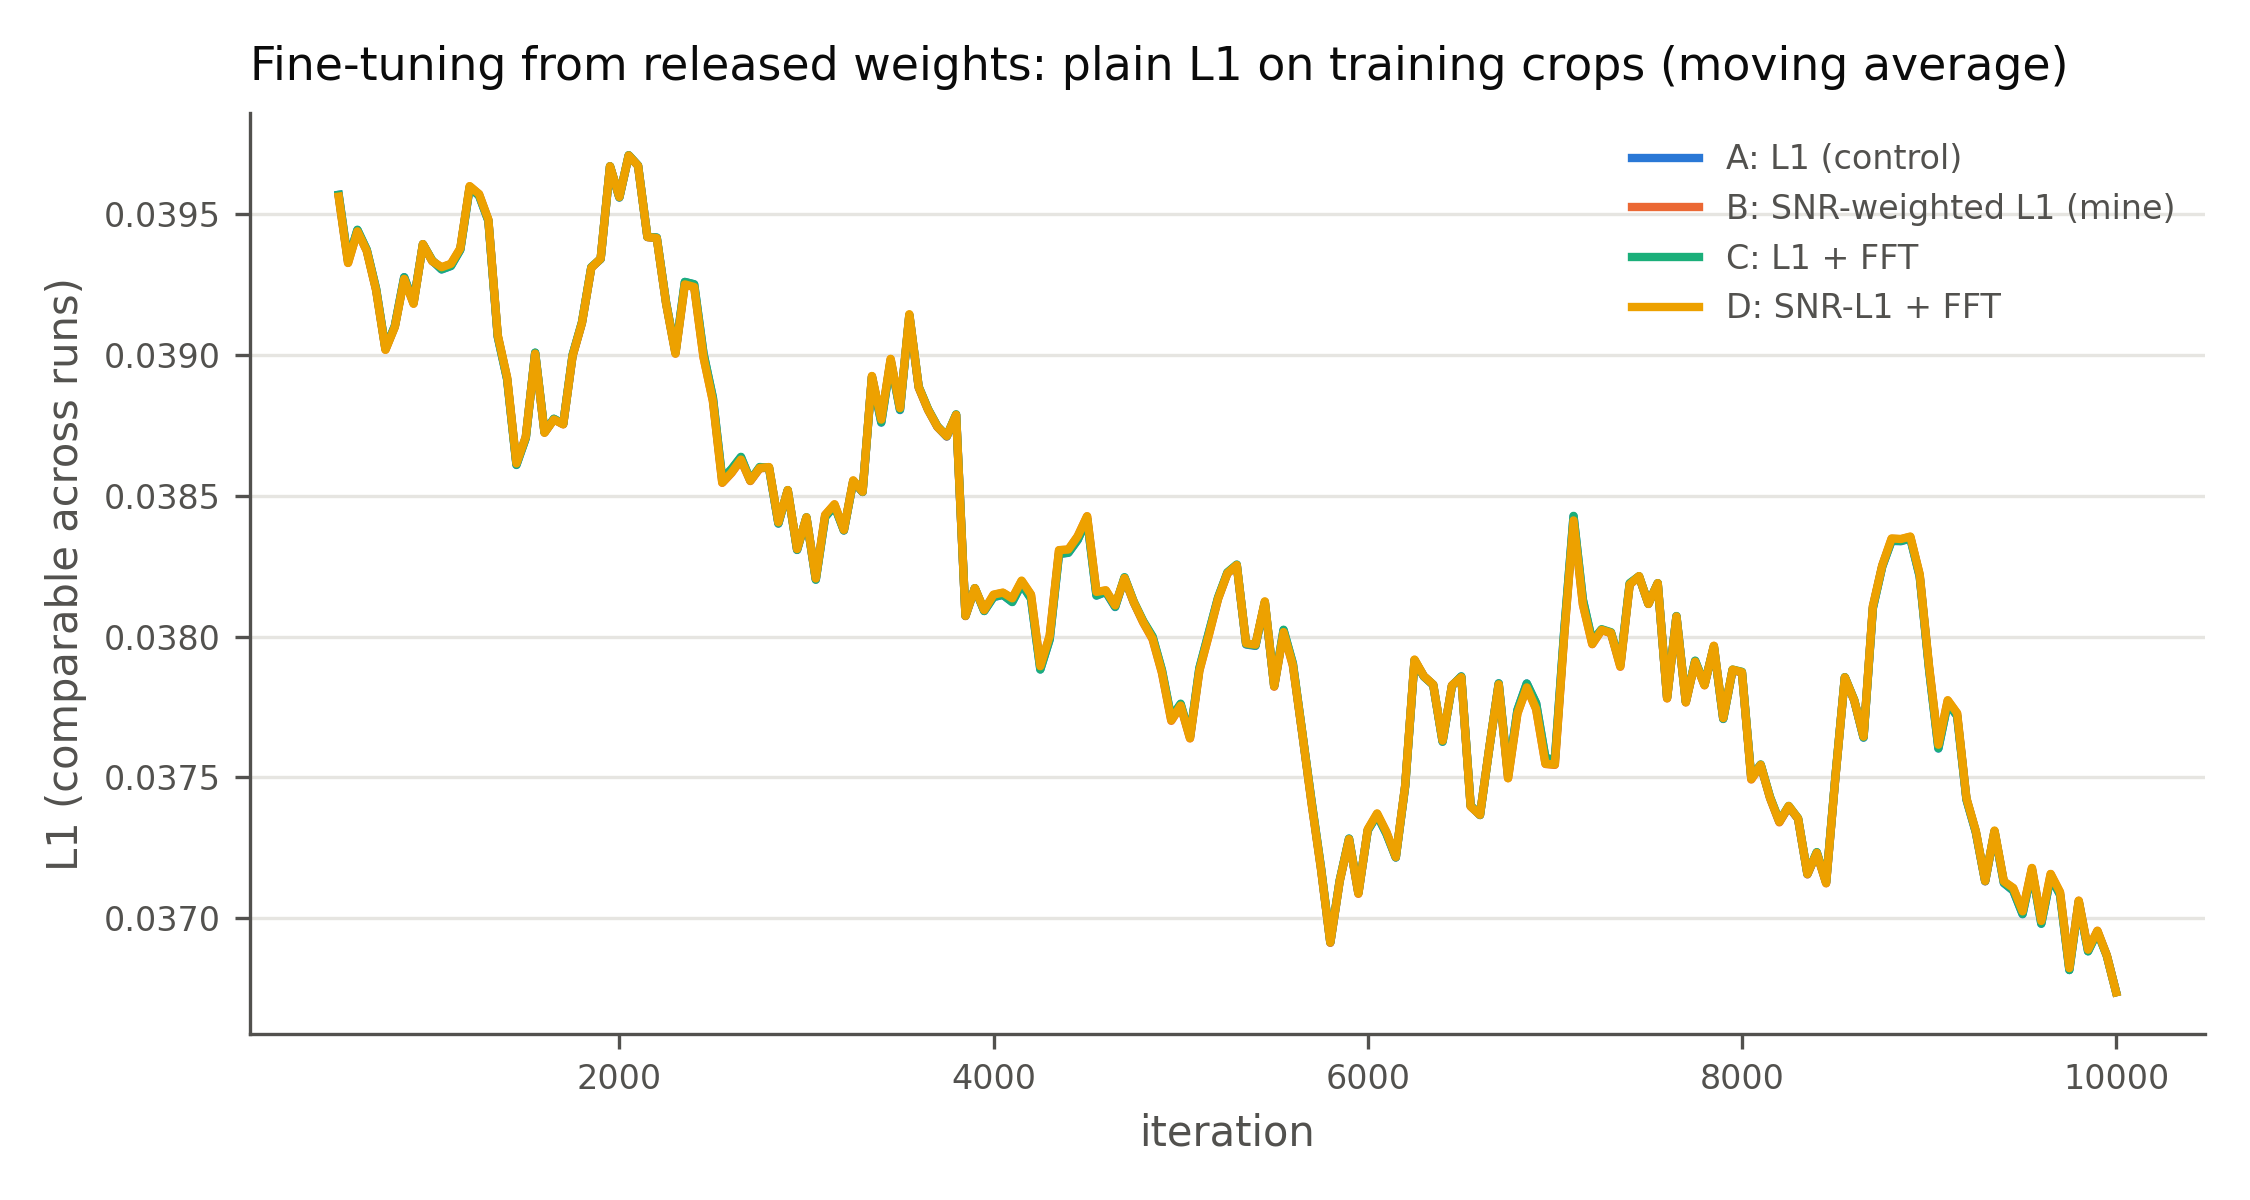
\includegraphics[width=\columnwidth]{finetune_curves.png}
\caption{Training $\ell_1$ during fine-tuning (moving average). The four curves overlap almost completely.}
\label{fig:ft}
\end{figure}

% =====================================================================================================
\begin{table}[t]
\centering
\caption{Plan for the second half of the semester}
\label{tab:plan}
\begin{tabular}{p{0.9cm} p{6.6cm}}
\toprule
Weeks & Work \\
\midrule
1--2 & SNR map as an additional guide in IG-MSA (e.g. scaling $V$ or masking attention by SNR); separate noise from edges (e.g. noise estimate on flat regions only) \\
3--4 & Sweep $\alpha$ and the weighting curve; 3 seeds per setting to measure run-to-run variance \\
5--6 & Train the best variant from scratch; evaluate on larger paired test sets (LOL-v2-syn, and SID/SMID if compute allows) \\
7 & Detection: fine-tune YOLOv8 on enhanced ExDark training images vs.\ raw; joint enhancement--detection objective if time allows \\
8 & Final report, code release \\
\bottomrule
\end{tabular}
\end{table}

\section{Discussion and Limitations}\label{sec:discussion}
\emph{What worked.} Running all methods through one protocol exposed effects that published tables hide: an evaluation
step that uses the ground truth, a train/test overlap between benchmarks, and the fact that better-looking images are
not better inputs for a detector trained on normal light.

\emph{Why the SNR loss had so little effect.} (i) The re-weighting is gentle by design: weights span 0.67--1.33, and
dark pixels receive on average only about 13\% more weight. (ii) The noise estimate $|g-\mathcal{B}_5(g)|$ cannot
distinguish noise from real detail: edges and textures also differ from their blurred version, so Fig.~\ref{fig:snr}(e)
puts high weights on edges as well as on noisy flat regions. (iii) Retinexformer's light-up features already tell the
network where the image is dark. (iv) Fine-tuning a converged model for 10k iterations at a small learning rate leaves
little room for any loss to change its behaviour.

\emph{Why fine-tuning lowered LOL-v1 PSNR.} The training loss improved in all runs while LOL-v1 test PSNR fell and
LOL-v2-syn rose. With 485 training images, extra training moves the model away from a released checkpoint that appears
unusually good---consistent with our re-training (23.10~dB) and the independent 23.45~dB report. Because A and B are
affected equally, the A--B comparison remains fair.

\emph{Limitations.} LOL-v1 has only 15 test images, so differences of a few tenths of a dB in average PSNR are not
meaningful; one random seed was used per run; training was limited by the free GPU quota (about 30 hours per week);
the detection study uses one detector without fine-tuning and ExDark labels are imperfect; GSAD was run on 200 ExDark
images only; SNR-Aware could only be evaluated on released images. Fig.~\ref{fig:fail} shows shared failures: text on a
bottle in image 493 is lost by every method, including ours.

\begin{figure}[t]
\centering
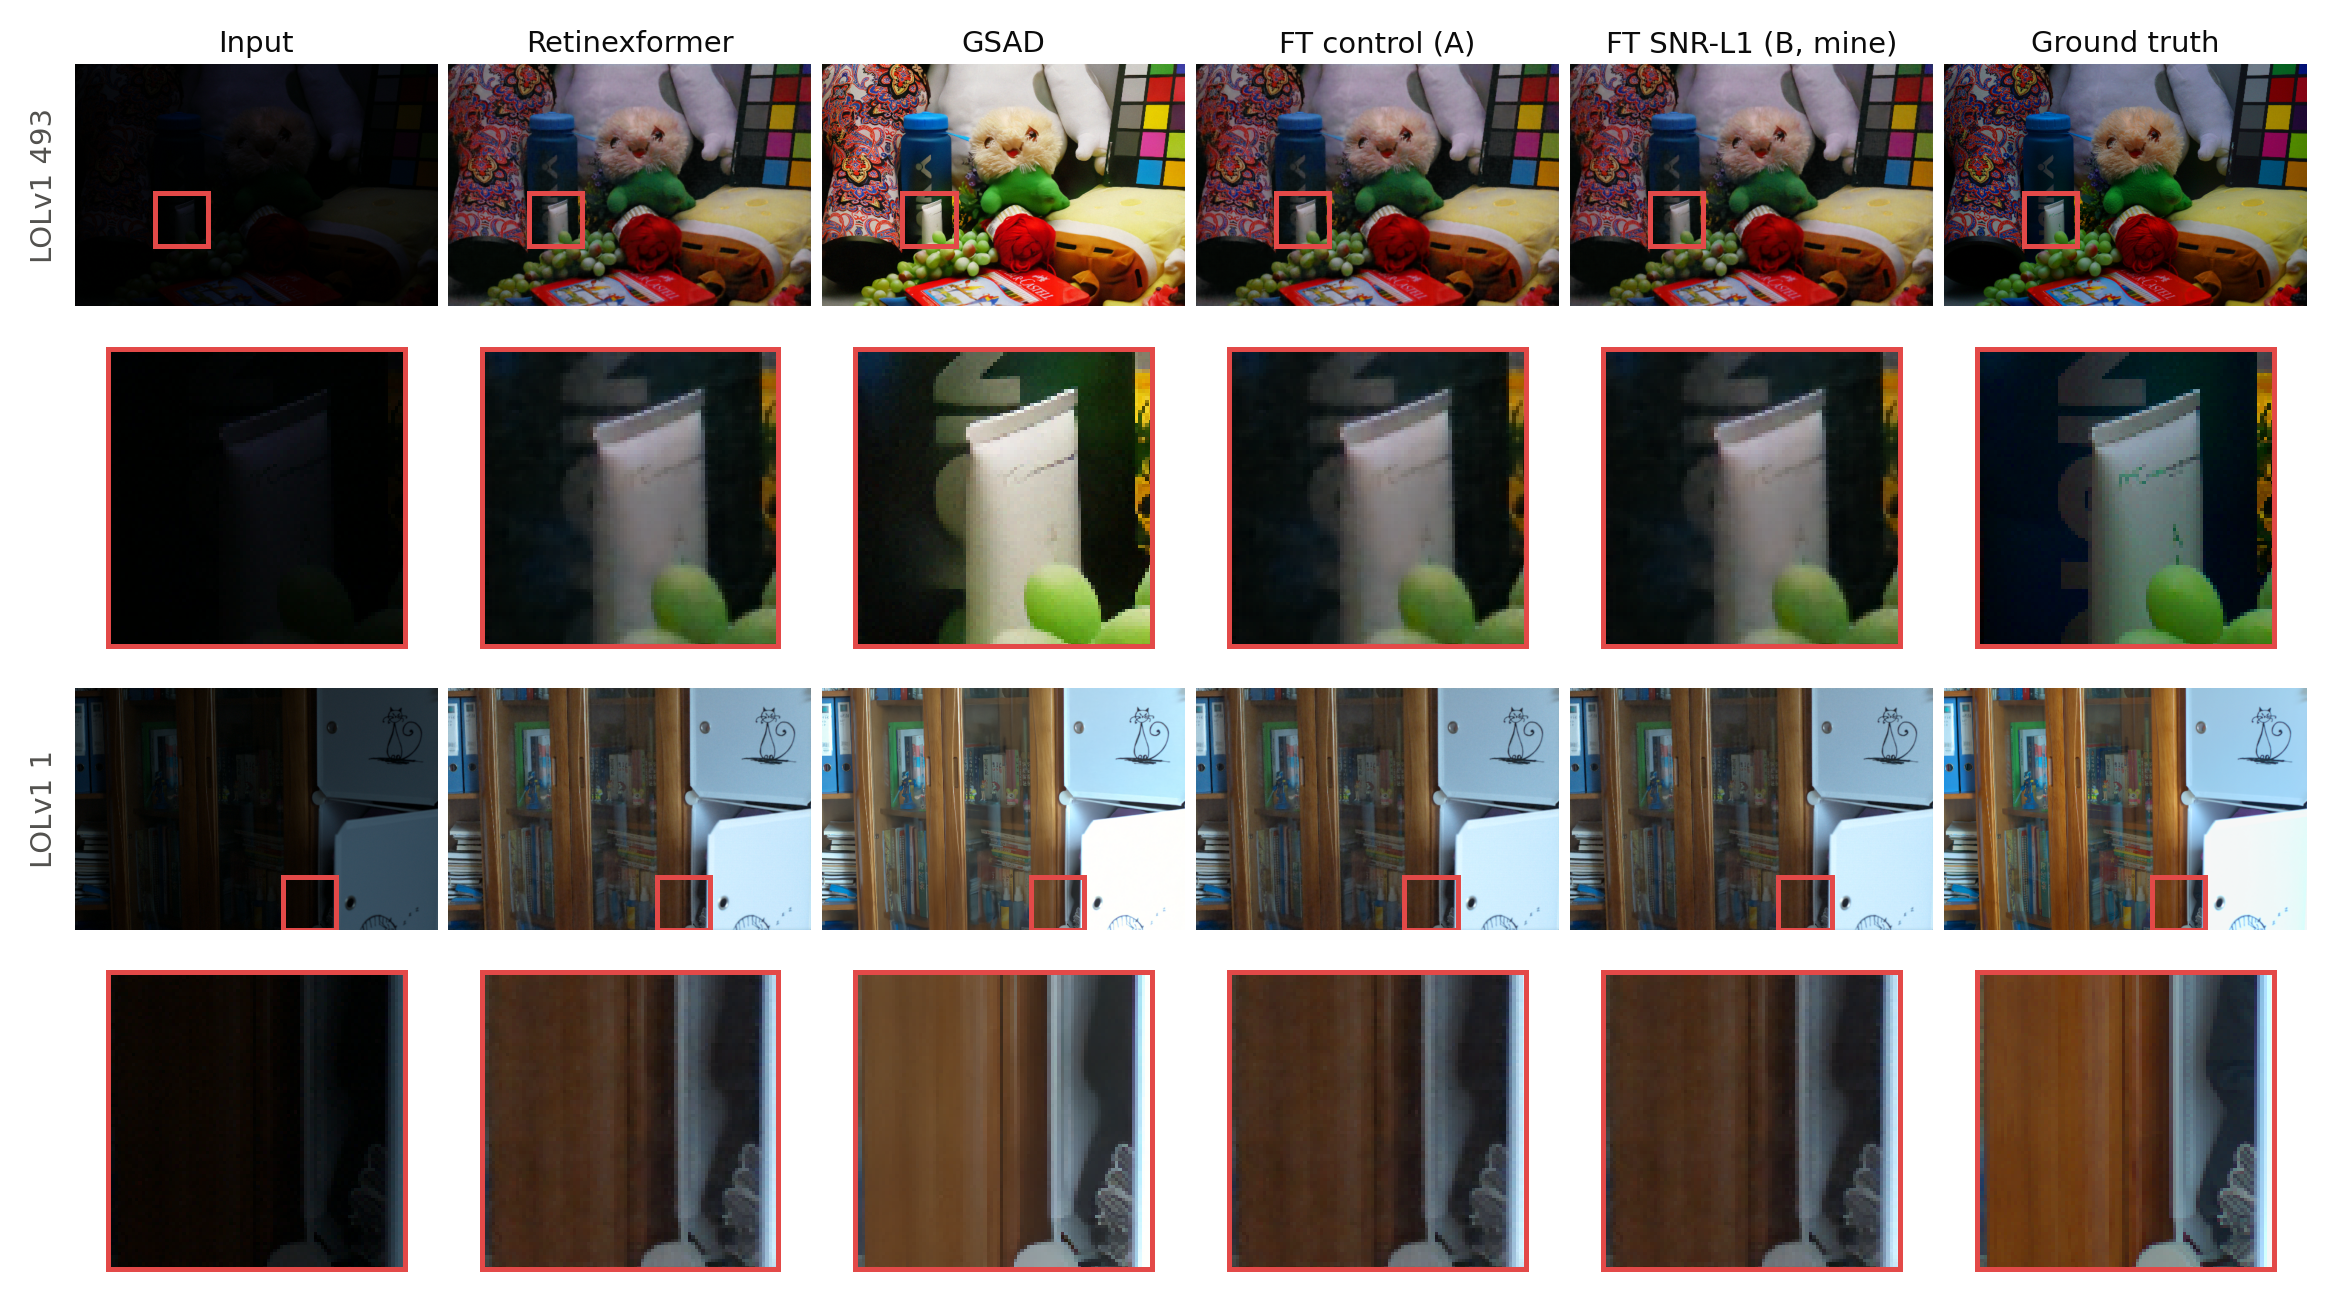
\includegraphics[width=\columnwidth]{failures_lolv1.png}
\caption{Failure cases on LOL-v1: fine text (493) and dark texture (1) are lost by all methods; GSAD adds a colour
cast. A and B are indistinguishable.}
\label{fig:fail}
\end{figure}

% =====================================================================================================
\section{Plan for the Remaining Semester}\label{sec:plan}
Table~\ref{tab:plan} lists the planned work. The main change of direction is to move noise awareness from the loss into
the network, where SNR-Aware showed it can matter, and to measure effects on test sets large enough to resolve them.


% =====================================================================================================
\section{Conclusion}\label{sec:conclusion}
We reproduced Retinexformer and eight baselines under one evaluation protocol and confirmed the published results of the
released models, while re-training from scratch fell about 2~dB short. The common protocol revealed that a diffusion
baseline's published numbers depend on a ground-truth brightness correction, that LOL-v2-real largely overlaps LOL-v1
training data, and that no enhancer helps a COCO-pretrained detector on ExDark. A noise-aware, SNR-weighted loss,
tested against a strict control, produced a consistent but negligible improvement in the darkest regions. The second
half of the project will move noise awareness into the attention mechanism and evaluate on larger test sets.

\FloatBarrier
\bibliographystyle{IEEEtran}
\bibliography{refs}

\end{document}
